Toda la información del presente capítulo ha sido obtenida de las diferentes fuentes que tiene la
Universidad de Chile tanto físicas como digitales que se especifican a lo largo del documento.
Además, se utilizó la información obtenida de una encuesta realizada a estudiantes, graduados
y académicos del Programas para enriquecer el informe y validar la información entregada en
diversos aspectos relativos al Programa. En varias secciones de este Capítulo nos referiremos a los
resultados de la encuesta pero sus detalles son presentados en la Sección \ref{encuestas} del presente informe.

\section{Definición Conceptual}

El Magíster en Ingeniería de Redes de Comunicaciones (en adelante mencionado
indistintamente por su nombre completo o como ``el Programa''), se encuentra en concordancia
con el Reglamento General de Estudios Conducentes a los Grados de Magíster y Doctor, Decreto
Universitario N$^\circ$~0028011 de octubre del año 2010 de la Universidad de Chile [\ref{reg_mag_doc}]. Este
Reglamento en su artículo 23 establece que:

\textit{``Un Programa conducente al grado de Magíster debe entregar conocimientos y competencias que
habiliten a los graduados para abordar asuntos complejos en forma sistemática y creativa. Estos
deben demostrar originalidad en la aplicación del conocimiento a través del planteamiento y la
resolución de problemas. Los Programas podrán orientarse al desarrollo de capacidades para:
La investigación, la innovación tecnológica, la creación artística o el desempeño profesional
superior.''}

En este contexto, el Programa se ha definido con el objetivo de ofrecer una formación profunda
en las redes de comunicaciones. Está diseñado para aquellas personas que deseen orientar
sus estudios hacia actividades principalmente de desarrollo y docencia superior. Es así como el
Programa corresponde a un Magíster de carácter profesional, presencial a tiempo completo y de
jornada vespertina. Esto es plenamente concordante con lo definido por la CNA para los Programas
de Magíster. 

% El Programa posee una articulación natural con la Carrera de Ingeniería Civil
%Eléctrica (ICE) de la Facultad de Ciencias Físicas y Matemáticas de la Universidad de Chile, del
%cual proviene un 71\% de sus estudiantes (ver Sección \ref{prog_eval}). Esta articulación permite que los
%estudiantes de ICE que postulen al grado de Magíster, ya sea simultáneamente o después de obtener
%su título profesional de Ingeniería, puedan convalidar UDs obtenidas por cursos de nivel 6000
%(electivos de la carrera de ICE) así como cursos electivos de nivel 7000 (electivos de postgrado).
%Se destaca el caso de los estudiantes que optan por doble titulación en el momento de realizar su
%trabajo de titulación en paralelo con la Tesis de Magíster, permitiendo en algunos casos el doble
%grado de Ingeniero y Magíster en 6 años y medio. Todo esto en concordancia con el Reglamento
%General de Magíster y Doctorado de la Universidad de Chile [\ref{reg_mag_doc}] y con el reglamento Interno
%de Magíster [A.8]. Asimismo, el carácter académico del Magíster permite la articulación con el
%Programa de Doctorado en Ingeniería Eléctrica en forma natural. Dicha articulación se desarrolla
%a nivel académico con estudiantes de Magíster que continúan en el Doctorado. Desde la Dirección
%del Departamento de Ingeniería Eléctrica los esfuerzos se han orientado a reforzar la sinergia
%del postgrado en el área eléctrica. Por lo anterior, desde el año 2012, los comités académicos
%del Magíster y el Doctorado se han fusionado para sesionar actualmente como un único Comité
%Académico de Postgrado del Departamento de Ingeniería Eléctrica.

\section{Contexto Institucional}
\label{contexto_institucional}

\subsection{Estructura Organizacional Institucional}

\subsubsection{Vicerrectoría de Asuntos Académicos}

Dentro de las vicerrectorías mencionadas en la Sección \ref{historia}, la Vicerrectoría de Asuntos
Académicos (VAA) tiene relación directa con la normalización de los planes de estudios de pre y
postgrado de la Universidad de Chile, la atención integral de los estudiantes, la selección y admisión
de alumnos, y las actividades de autoevaluación institucional, entre otras.

Su ámbito de trabajo cubre todo el espectro de la vida académica y de formación integral de
los estudiantes de pregrado y postgrado, incluyendo la selección y admisión de alumnos a través
de la PSU para todo el sistema universitario. Con una perspectiva de aseguramiento de calidad,
y en colaboración con las unidades académicas, define políticas para el desarrollo, creación y
modernización de los Programas de estudios de Pre y Postgrado, así como en el otorgamiento
de servicios académicos de bienestar y de recreación a los estudiantes atendiendo a su equidad.

Además, la Vicerrectoría presta apoyo técnico a las Facultades, Escuelas e Institutos
principalmente en su gestión curricular y procesos de acreditación, y mantiene información
actualizada de la calidad académica de la Universidad.

Según el articulo 16 del Reglamento General de Estudios Conducente a los Grados de Magíster
y Doctor (Decreto Universitario N$^o$0028011 de 5 de octubre de 2010) [\ref{reg_mag_doc}], la VAA velará
por la calidad de los Programas de postgrado, sometiéndolos a acreditación interna y externa,
estableciendo los organismos y procedimientos para cada caso. En particular según el articulo 17
del mismo reglamento, para efecto de la acreditación interna la VAA deberá considerar, al menos:

\begin{itemize}
\item Idoneidad y tamaño del claustro de profesores del Programa;
\item Líneas de investigación que sustenten el Programa;
\item Efectividad del proceso de enseñanza aprendizaje;
\item Coherencia entre los objetivos del Programa, el perfil de graduación y sus resultados;
\item Infraestructura y disponibilidad de servicios y recursos educacionales, y
\item Mecanismos implementados para el aseguramiento de la calidad.
\end{itemize}

En lo referente a Postgrado, la Vicerrectoría de Asuntos Académicos posee un Departamento
de Postgrado y Postítulos (DPP). Este tiene como finalidad cautelar y estimular el desarrollo de
los estudios conducentes a los grados de Magíster y Doctorado, y de cursos de especialización
profesional en todas las unidades académicas del plantel. De igual forma, articula los recursos
humanos y materiales en relación a la creación de nuevos grados académicos y cautela la idoneidad
y calidad de los Programas que ofrece la Casa de Estudios.

En este sentido el DPP trabaja en estrecha relación con la Escuela de Postgrado de la FCFM,
así como con las otras unidades del área académica de la Vicerrectoría de Asuntos Académicos,
con la Vicerrectoría de Investigación y Desarrollo, y la Dirección de Relaciones Internacionales
(dependiente de Rectoría) de la Universidad de Chile.

En cumplimiento de su misión, brinda asistencia en la formulación, revisión y actualización
de Programas de Magíster y Doctorado y de especialización profesional, y homogeneiza normas y
reglamentos atingentes a la materia. Por otra parte, administra la asignación de recursos de becas
para estudiantes meritorios y desarrollo de tesis.
Asimismo promueve el ingreso de alumnos extranjeros a los Programas de postgrado y de
especialización.

\subsubsection{Acreditación Institucional 2011 - 2018}

%El 21 de diciembre de 2011 la Universidad de Chile recibió oficialmente la acreditación
%institucional por parte de la Comisión Nacional de Acreditación - CNA, por el periodo máximo
%de tiempo de siete años -hasta el 21 de diciembre de 2018- tras registrar positivas evaluaciones
%en todas las áreas de evaluación, tanto aquellas obligatorias -gestión institucional y docencia de
%pregrado- como en aquellas electivas -investigación, docencia de posgrado y vinculación con el
%medio-. Esto fue expuesto en el Acuerdo N$^o$161 de la Comisión Nacional de Acreditación CNA
%[A.9].

%Se destaca en el área de docencia de Postgrado (extraído del acuerdo N$^o$ 161 de la CNA):

%\begin{itemize}
%\item Se registra un claro liderazgo Institucional en el área de Postgrado y una numerosa oferta
%de Programas de calidad, cuya provisión se encuentra debidamente normada mediante
%la existencia de políticas y mecanismos que regulan su oferta. En especial se destacan
%los mecanismos de aseguramiento de calidad de los Programas de doctorados, los cuales
%presentan una importante contribución social a nivel nacional.
%\item La universidad presenta infraestructura física, biblioteca y servicios estudiantiles adecuados
%para la oferta de Programas de postgrado. Asimismo, se constata la existencia de mecanismos
%de aseguramiento de la calidad de la docencia, lo cual permite contar con académicos de
%destacado nivel.
%\item Se constata la existencia de una rica actividad académica, la cual es alimentada por visitas
%de profesores, intercambios estudiantiles, realización de tesis en co-tutela, pasantías y
%convivencia con investigadores de post doctorado. Igualmente se evidencia un claro traspaso
%de las actividades investigativas a la docencia de postgrado. La generación de publicaciones
%a nivel internacional y la participación de los estudiantes en dichas actividades son un claro
%ejemplo de aquello.
%\end{itemize}

%Se destaca en el área de Investigación (extraído del acuerdo N$^o$ 161 de la CNA):
%\begin{itemize}
%\item La Universidad de Chile presenta una tradición de cultivo de la investigación, siendo esta
%característica parte esencial de su ser universitario. Asimismo, presenta una alta calidad en
%su producción científica en relación a estándares nacionales e internacionales. De esta forma,
%la Universidad de Chile se sitúa en una posición de liderazgo a nivel nacional, cuenta con
%gran prestigio al respecto e impacta, con sus investigaciones, en el desarrollo del país.
%\item El quehacer investigativo de la Universidad permea todas las actividades institucionales.
%Se evidencia, especialmente, una importante vinculación con la docencia de postgrado; en
%particular lo que respecta a la interrelación con los Programas de doctorado y magísteres
%académicos.
%\end{itemize}

\subsubsection{Escuela de Postgrado}

El enlace de los Programas de Postgrado de la FCFM con la institucionalidad pertinente
(Departamento de Postítulo y Postgrado de la Universidad de Chile (DPP)) es a través de la Escuela
de Postgrado. Esta tiene como función organizar, administrar e impartir los estudios conducentes
a la obtención de grados académicos de Magíster y Doctor. Su máxima autoridad es su Director,
quien en conjunto con el Consejo de la Escuela de Postgrado pondrán en práctica las políticas de
desarrollo de la docencia de postgrado.

La Escuela de Postgrado asegura el funcionamiento operacional y académico de todos los
Programas de Postgrado de la FCFM. Además permite la sinergia de los mismos, la construcción
de criterios comunes, el crecimiento orgánico y el mejoramiento continuo.

\subsubsection{Normativas y Reglamentos}

El Programa se rige por los reglamentos de la Universidad de Chile nombrados a continuación y
que se adjuntan en los anexos respectivos.

El principal reglamento de postgrado de la Universidad de Chile es el Reglamento General
de Estudios Conducentes a los Grados de Magíster y Doctor [\ref{reg_mag_doc}]. Además posee un reglamento
general propio del Programa [\ref{reg_mirc}].

Dada la naturaleza de la Universidad de Chile, se exige tener un reglamento general con
las características definidas para éste, pero además se hace necesario y recomendable tener un
reglamento interno donde se estipulan, entre otros temas, los requisitos operativos y de gestión del
Programa. Actualmente se encuentra vigente el reglamento general del Programa del año 2006.
Además, está en fase de tramitación en los cuerpos colegiados de la Universidad de Chile, el nuevo
reglamento general del Programa, ambos en el Anexo correspondiente [\ref{reg_mirc}].

La estructura reglamentaria de la Universidad de Chile es clara en lo que respecta a los
Programas conducentes a los grados de magister y doctorado [\ref{reg_mag_doc}]. Esta reglamentación define
un marco sobre el cual se regulan los Programas tocando aspectos tales como la naturaleza del
Programa, sus objetivos y perfil de graduación, su creación, la administración, la conformación
del claustro, las responsabilidades del comité académico, las responsabilidades de la escuela
de postgrado, la acreditación y procesos de aseguramiento de calidad. Adicionalmente en este
Reglamento hay disposiciones específicas para los Programas de Magister que tocan aspectos
relativos a postulación y criterios de selección, plan de formación, proyecto de grado, actividad
de graduación, extensión mínima y máxima del Programa, homologación de UDs, criterios de
aprobación, entre otros. Complementando lo anterior el Programa consta de un Reglamento
General [\ref{reg_mirc}]. El primero establece aspectos reglamentarios
específicos que definen con mayor precisión el Programa, en el marco del Reglamento General de
la Universidad de Chile. Un ejemplo de ello es la definición concreta de los objetivos del Programa,
su plan de formación y su extensión en lo que respecta a número de UDs. Dichos reglamentos son
coherentes entre si y además deben ser revisados por el área jurídica de la Universidad así como
aprobados por los cuerpos colegiados respectivos. Finalmente, el Reglamento Interno se hace cargo
de las disposiciones operativas del Programa, como son, por ejemplo, estipular el Programa de
ayuda de viajes y los criterios arancelarios. Los Reglamentos Generales e Internos del Programa
se actualizan y revisan periódicamente por el Comité Académico del Programa, como se evidencia
en la renovación de los mismos en los últimos años.

\subsection{Sistema de Organización Interna}

\subsubsection{Organigrama del Departamento de Ingeniería Eléctrica}

El Departamento de Ingeniería Eléctrica de la Universidad de Chile tiene por su parte una
organización autónoma que vela por el buen funcionamiento tanto de la carrera de Ingeniería Civil
Eléctrica como de los Programas de postgrado (ver Fig. 2.1).

\begin{figure}[ht]
\centering
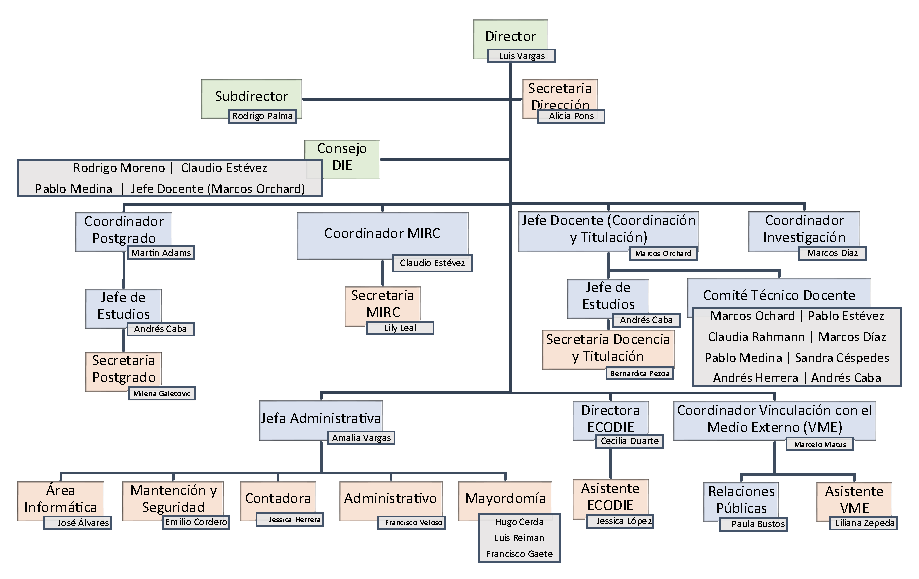
\includegraphics[width=\columnwidth]{./organigramas/die.eps}
\caption{Organigrama del Departamento de Ingeniería Eléctrica.}
\label{orga_die}
\end{figure}

Las funciones de Director de Departamento corresponderán a quien sea elegido por sus
académicos (jornada completa y parcial) conforme al Reglamento General de Elecciones y
Consultas [\ref{reg_elec_cons}], quien deberá ser un académico de las dos más altas jerarquías. Para cumplir
sus funciones deberá contar con una jornada contratada no inferior a 22 horas. Durará dos años en
sus funciones pudiendo ser reelegido por un periodo adicional.

El Reglamento General de Facultades [\ref{reg_gen_fac}] define las responsabilidades del Director de
Departamento como sigue:

\begin{enumerate}
\item Representar al Departamento ante el Consejo de Facultad y ante otras instancias.
\item Presidir el Consejo del Departamento.
\item Proponer al Decano la celebración de contratos de prestación de servicios y convenios de
honorarios.
\item Coordinar con los Directores de Escuela la realización de actividades de docencia que
correspondan al Departamento, para asegurar la calidad de la docencia impartida por los
miembros de su Departamento.
\item Presentar al Consejo del Departamento, para su aprobación, los planes anuales de desarrollo
académico de Departamento y su presupuesto, velando por su cumplimiento.
\item Entregar un informe fundado de las actividades de los académicos de su Departamento a la
Comisión de Calificación de su Facultad, con conocimiento por parte de cada interesado.
\item Presentar al Decano una cuenta anual sobre el funcionamiento académico y financiero del
Departamento para que éste la presente al Consejo de Facultad.
\item Proponer al Decano, con la aprobación del Consejo del Departamento, el nombre de la persona
que desempeñará la función de Subdirector, el cual colaborará en su gestión y lo subrogará en
caso de ausencia o impedimento. El subdirector deberá ser un académico de la categoría de
Profesor.
\item Determinar la creación de coordinaciones de apoyo a la Dirección cuando lo estime conveniente,
así como el nombre de las personas que desempeñarán esas funciones.
\item Las demás que le fija la reglamentación universitaria o que el Decano le delegue.
\end{enumerate}

El Consejo del Departamento se conforma por 6 académicos, 2 de ellos son parte de éste
por derecho propio (Director y Jefe Docente) y 4 son elegidos por el claustro académico. Los
consejeros de libre elección duran dos años en sus funciones, pudiendo ser reelegidos. Pueden
participar también, como invitados, representantes estudiantiles cuando las materias lo ameriten y
son elegidos de acuerdo a lo establecido por su organización estudiantil de Facultad.

Según el Reglamento General de Facultades [\ref{reg_gen_fac}] corresponde al Consejo de Departamento:

\begin{itemize}
\item Aprobar el plan anual de desarrollo académico y el presupuesto correspondiente.
\item Aprobar la proposición de un académico, hecha por el Director de Departamento, para que
aquél cumpla la función de Subdirector. Una vez aprobada, será propuesta al Decano.
\item Aprobar los planes de gestión de proyectos y servicios que someta a su consideración el
Director de Departamento.
\item Las demás que le asignen los reglamentos o que le encomiende el Director del Departamento.
\end{itemize}

El Subdirector cumple la función de subrogar al Director del Departamento en caso de
ausencia o impedimento de este.

La Oficina Administrativa controla, gestiona y ejecuta el presupuesto de la Unidad. La
Oficina Administrativa reporta a la Dirección Económica y Administrativa de la FCFM. Además
de los sueldos y remuneraciones, esta oficina gestiona la contratación de profesores part-time y
profesionales, los recursos de unidades de beca para el pago de auxiliares y ayudantes docentes,
adquisición de material bibliográfico, adquisición de equipamiento computacional y de laboratorio,
recursos de educación continua, y recursos de titulación y graduación. Además gestiona los
recursos humanos de la unidad, en particular mayordomos, estafeta, encargado de mantención
y electricidad, encargado de laboratorios docentes, encargado de taller mecánico. El Jefe
administrativo se selecciona en base a concurso público y la decisión para su selección es colegiada
y cuenta con la participación de las más altas autoridades administrativas de la Facultad. La actual
jefa administrativa del DIE es de profesión ingeniera comercial.

El Jefe Docente es nominado por el Director de Departamento y ratificado por el Decano.
Dentro de sus funciones está liderar el Comité Técnico Docente y participar en el Consejo de
Escuela. El Jefe Docente coordina todas las instancias relativas a la docencia de Ingeniería
Civil. Además está a cargo de la parte operativa, incluyendo atención de alumnos, solicitudes,
Programación de cursos, designación de profesores, etc. La implementación en el año 2007 de la
reforma curricular sumado a los procesos de acreditación y vertiginoso mercado laboral, exigen
una continua revisión de planes y Programas de estudio. Es por esto que como una forma de apoyar
la labor de los jefes y coordinadores docentes, cuyas funciones más urgentes tienen que ver con
la administración y gestión de la docencia, la Facultad de ciencias Físicas y Matemáticas propone
la conformación en cada departamento de Comités Técnicos Docentes (CTD), que con una mirada
integral de la carrera, apoyen el mejoramiento continuo de la docencia en el pregrado de la facultad,
contando con la asesoría de especialistas del Área de Desarrollo Docente (ADD) de la Escuela de
Ingeniería y Ciencias.

El Comité Técnico Docente (CTD) es elegido por el Jefe Docente y se conforma por al menos
2 académicos jornada completa (incluyendo al Jefe Docente), un académico de Jornada Parcial, y
al menos un estudiante de pregrado o postgrado.

El Jefe de Estudios cumple funciones administrativo académicas tanto en pregrado como en
postgrado. Su misión es apoyar en sus funciones al Jefe Docente y al coordinador de Postgrado.
El Coordinador de Innovación y Desarrollo potencia y lleva a cabo actividades relativas
a innovación y desarrollo tanto a nivel de departamento como con la interrelación con otros
departamentos de la Universidad de Chile.

El Coordinador de Educación Continua es el encargado de desarrollar y coordinar las
acciones de extensión del departamento. A su cargo está el EcoDie, unidad de educación continua
del departamento.

El Coordinador de Investigación enlaza y coordina las actividades de investigación de los
académicos del departamento.

Finalmente el Coordinador de Postgrado, así como el comité Académico de Postgrado, se
detallan a continuación en la sección de Gestión interna del Programa de Magíster. Tal como se
mencionó anteriormente, el Coordinador de Postgrado se apoya fuertemente en el Jefe de estudios
para la administración eficiente de los Programas.

\subsubsection{Gestión interna del Programa de Magíster Profesional}

El Programa de Magíster en Ingeniería de Redes de Comunicaciones, es administrado por la
Escuela de Postgrado de la Facultad de Ciencias Físicas y Matemáticas de la Universidad de Chile.
De acuerdo al Reglamento General de Estudios Conducentes a los Grados de Magíster y Doctor,
Decreto Universitario No0028011 de octubre del año 2010, de la Universidad de Chile [\ref{reg_mag_doc}], la
Facultad de Ciencias Físicas y Matemáticas de la Universidad de Chile debe poseer una Escuela
de Postgrado, la cual se encarga de la administración académica de los Programas de magíster
y doctorado. Para efectos de dicha administración, la Escuela de Postgrado es dirigida por un
Director, con la colaboración del Consejo de Escuela y el Comité Académico del Programa de Magíster en Ingeniería de Redes de Comunicaciones.

Dentro del DIE, el Programa cuenta con un Comité Académico, cuyos integrantes son
nombrados por el Director de Escuela, a proposición del claustro académico, y con el acuerdo
del Consejo de la Escuela de Postgrado de la FCFM. Este Comité Académico está conformado por
al menos tres profesores pertenecientes al claustro académico del Programa, quienes eligen a uno
de ellos como Coordinador. Los miembros del Comité Académico duran dos años en sus funciones,
pudiendo ser nominados por otros períodos.

En concordancia con el Reglamento General de Estudios Conducentes a los Grados de
Magíster y Doctor de la Universidad de Chile [\ref{reg_mag_doc}] en sus articulos 6 y 7, el Comité Académico se
responsabiliza por gestionar los aspectos académicos del Programa, velando por el cumplimiento
de sus objetivos, por el mejoramiento continuo del Programa y por la formación de sus estudiantes,
de acuerdo a estándares de calidad establecidos por la Universidad de Chile.

Las funciones del Comité Académico son:

\begin{itemize}
\item Seleccionar a los estudiantes que se incorporarán al Programa
\item Aprobar los planes de estudios de los postulantes
\item Nombrar a los respectivos profesores guías 
\item Aprobar al profesor guía de la tesis propuesto por cada estudiante
\item Proponer al Director de Escuela los integrantes de la comisión evaluadora de proyectos de
tesis, de la tesis y del examen de grado
\item Elaborar periódicamente un informe sobre el estado del Programa a su cargo, verificando el
cumplimiento de los indicadores de calidad definidos por la Facultad, y
\item Cautelar que la investigación que realicen los estudiantes considere las normas y
procedimientos propios de la disciplina.
\end{itemize}

Para estos efectos, el Comité Académico se sesiona periódicamente para analizar, debatir
y resolver sobre las distintas responsabilidades mencionadas anteriormente. En el último ano
el Comité ha sesionado a una tasa promedio de dos reuniones menusuales. Por otra parte, el
involucramiento del resto del claustro académico en términos de gestión y academia, radica en
buena medida en su rol como guias de tesis. No obstante, se realizan jornadas periódicas
a lo largo del año con el resto del claustro con el fin de formar un espacio para la discusión y el
debate en torno a las materias del Programa. En general el funcionamiento propende a la integración
total y continua del claustro en el desarrollo del Programa.

% En cuanto al fortalecimiento de la gestión diaria, atención de estudiantes, apoyo a profesores,
% manejo administrativo, entre otros, en los últimos años se ha impulsado el desarrollo del cuerpo de
% profesionales involucrados en la gestión del magíster y doctorado, así como la homologación de
% funciones de gestión interna en el departamento. En este contexto destacan los siguientes hitos:

% \begin{itemize}
% \item Fusión de los Comités Académicos de magíster y doctorado. Desde el año 2011 y en pos de
% una articulación cada vez más eficiente, se fusionaron los comités de Magíster y Doctorado
% del departamento.
% \item Contratación del Jefe de Estudios del Departamento de Ingeniería Eléctrica en Diciembre del
% 2014. Como se mencionó en la sección anterior, el Jefe de Estudios apoya las labores del
% Jefe Docente y del Coordinador de Postgrado. En virtud de lo anterior, este cargo potencia la
% articulación de la carrera de pregrado con el postgrado del Departamento.
% \item Contratación de una Secretaria de Postgrado en Diciembre del 2014. Este cargo fusiona las
% responsabilidades de la secretaria de magíster y secretaria de doctorado.
% \end{itemize}

% Cabe destacar de estas contrataciones el perfil requerido, donde se hizo especial hincapié en
% que dichos profesionales contaran con una amplia trayectoria en gestión universitaria. Se destaca
% además que la secretaria de Postgrado cuenta con estudios formales de idiomas.

\section{Características y Resultados del Programa}

\subsection{Carácter, objetivos y perfil de egreso}

\subsubsection{Definición del Programa}

El Magíster en Ingeniería de Redes de Comunicaciones, es un Programa de carácter profesional que, esencialmente, 
fue creado para formar a estudiantes en el área de redes de comunicaciones. 
Su plan de formación apunta a que los estudiantes se formen en tópicos
avanzados de telecomunicaciones y redes de comunicaciones. Esto les permite desarrollarse en la frontera del conocimiento
a través del ejercicio mismo del desarrollo que realizan bajo la cercana supervisión de los
profesores guías de tesis.

El Programa se encuentra perfectamente alineado con el perfil que establece la Universidad de
Chile. Este perfil se define explícitamente a través del Reglamento General de estudios conducentes
a los grados de Magíster y Doctor [\ref{reg_mag_doc}]. En su artículo 23, el reglamento estipula:

``Un Programa conducente al grado de Magister debe entregar conocimientos y competencias que
habiliten a los graduados para abordar asuntos complejos en forma sistemática y creativa. Estos
deben demostrar originalidad en la aplicación del conocimiento a través del planteamiento y la
resolución de problemas. Los Programas podrán orientarse al desarrollo de capacidades para: la
investigación, la innovación tecnológica, la creación artística o el desempeño profesional
superior.''

Por tanto, el Programa está dirigido a aquellas personas que deseen orientar sus estudios hacia
las actividades de innovación, desarrollo y docencia superior, en la disciplina de
Ingeniería Eléctrica con especialidad en Redes de Comunicaciones.

El Programa se rige por el reglamento General del Programa [\ref{reg_mirc}]. 
Dada las normas de la Universidad de Chile, se exige que los progamas tengan
un reglamento general que contenga las definiciones básicas del Programa. Adicionalmente es
necesario y recomendable contar con un reglamento interno donde se estipulan, entre otros temas,
los requisitos operativos y de gestión del Programa.

\subsubsection{Perfil de egreso}

\noindent\textbf{Objetivo general}

El Magister en Ingeniería de Redes de Comunicaciones (MIRC), de la Universidad de Chile, 
es un postgrado orientado a profesionales del área de tecnologías de comunicaciones que 
les permite profundizar y aplicar el conocimiento de redes de comunicaciones de última 
generación, gestión de proyectos de alta integración tecnológica, estudio de la economía 
que rodea a las telecomunicaciones, regulación chilena de las telecomunicaciones y la 
seguridad de las redes de comunicaciones. Este Programa equilibra aspectos teóricos, 
otorgando una sólida base conceptual en redes de comunicaciones, con factores imprescindibles 
en el ámbito profesional que habilitan al egresado a poner en práctica dicho conocimiento.

\noindent\textbf{Objetivos específicos:}

\begin{itemize}
\item Entregar una sólida base teórica sobre redes de comunicaciones y su aplicación en tecnologías 
inalámbricas, redes móviles y redes de banda ancha.
\item Formar profesionales que puedan reconocer tecnologías aplicadas de última generación para 
luego aplicarlas hábilmente en su medio laboral.
\item Entregar las herramientas para que puedan identificar y solucionar problemas de seguridad 
en redes complejas. 
\item Enseñar a gestionar calidad en redes móviles, formulando, diseñando y aplicando modelos de 
calidad de experiencia.
\item Habilitar el desarrollo de competencias profesionales necesarias para evaluar alternativas 
técnico-económicas, diseñar y gestionar proyectos tecnológicos y liderar iniciativas tecnológicas de punta.
\end{itemize}

\noindent\textbf{Descripción del Perfil de Egreso:}

Los graduados del Magíster en Ingeniería de Redes de Comunicaciones (MIRC) son profesionales habilitados para:

\begin{itemize}
\item Demostrar originalidad en la aplicación del conocimiento a través del planteamiento y la resolución de problemas en los siguientes ámbitos:
\begin{itemize}
\item Comunicación digital y analógica
\item Interconexión de redes
\item Redes multiservicios (incl. Cloud computing, IoT, Big Data, etc.)
\item Redes Inalámbricas (incl. móviles)
\item Desempeño de redes de comunicaciones
\item Gestión de proyectos de redes.
\end{itemize}
\item Adaptar, operar y gestionar redes de comunicaciones sobre la base de una capacidad analítica y sólidas bases en aspectos teóricos y aplicados. 
\item Conocer aspectos de regulación y economía de las telecomunicaciones.
\item Liderar, gestionar e implementar proyectos de redes de comunicaciones de última generación.
\end{itemize}

\noindent\textbf{Perfil de Egreso:}

Los graduados del Magíster en Ingeniería de Redes de Comunicaciones son profesionales capaces 
de aplicar el conocimiento a través del planteamiento y la resolución de problemas en el ámbito 
de las redes de comunicaciones. Los alumnos graduados poseen los conocimientos necesarios para 
la comprensión de nuevas tecnologías de comunicaciones a medida que surgen. También están preparados 
para adaptar, operar y gestionar redes de comunicaciones sobre la base de una capacidad analítica y 
sólidos fundamentos en aspectos teóricos y aplicados. Así mismo, están habilitados para liderar, 
gestionar e implementar proyectos de redes de última generación. Se espera que tengan conocimientos 
de regulación y economía orientado a las telecomunicaciones. Los egresados están preparados para 
realizar labores en el ámbito de las redes de comunicaciones y organismos regulatorios. 


\subsubsection{Revisión y difusión del perfil de egreso}

Los mecanismos de revisión y difusión del perfil de egreso, así como del carácter y los objetivos del
Programa, son continuos y diversos. Se posibilitan y ejecutan a través de las siguientes instancias
formales:

\begin{itemize}
\item Reuniones regulares del Comité Académico. 
\item Reuniones del subcomité encargado del Perfil de Egreso.
\item Revisión por parte del claustro y colaboradores del Programa.
\end{itemize}

Adicionalmente, la unidad de Gestión Curricular de la FCFM apoya los procesos de revisión
de los perfiles de egreso de Postgrado y Pregrado. Además, apoya el desarrollo curricular de las
carreras y Programas de Postgrado.

El perfil de egreso es también validado a través del contacto con alumnos y egresados,
utilizando encuestas. En particular, la última encuesta realizada producto del presente proceso
de auto evaluación (ver Sección \ref{caract_obj_perf_egr}) señala que:

\begin{itemize}
% \item En promedio, los egresados y alumnos activos del Programa, está muy
% de acuerdo o de acuerdo con que el Programa tiene objetivos claros y conocidos.
\item En promedio, los egresados y alumnos activos del Programa, está 
de acuerdo con que el Programa contaba con un perfil de graduación claro.
\item En promedio, los egresados y alumnos activos del Programa están marginalmente de acuerdo con que 
los objetivos son congruentes con el enfoque del Programa.
\item En promedio, los egresados y alumnos activos del Programa están marginalmente 
de acuerdo con que el perfil de graduación era conocido.
% \item El <.#cap2_perfil(5,4)#.>\% de los egresados y alumnos activos del Programa, está muy de
% acuerdo o de acuerdo con que el perfil de egreso logró dar cuenta de los objetivos del Programa.
\end{itemize}

%El análisis de los tiempos de egreso oportuno, así como de las publicaciones de los estudiantes
%del Programa (ver Sección 2.3.4.2), son insumos cruciales para retroalimentar el análisis y lograr
%el mejoramiento continuo. Además, en pos de la mejora continua, la FCFM está actualmente
%desarrollando una nueva reglamentación del Magíster [A.18]. Este proceso es liderado por la
%Escuela de Postgrado, dentro del marco institucional de desarrollo de los Programas de Postgrado.
%En este mismo ámbito, se están actualizando el Reglamento General y el Reglamento Interno del
%Programa de <@programa@>.

Es importante también tener en cuenta que, reglamentariamente, se reconoce la importancia de
la revisión del perfil de egreso y el plan de formación del Programa. Según el Reglamento General
de estudios conducentes a los grados académicos de Magíster y Doctorado [\ref{reg_mag_doc}], en su artículo 17,
se dice que:

``El Comité Académico del Programa deberá elaborar, al menos cada cinco años, un informe
de autoevaluación considerando las directrices de la Vicerrectoría correspondiente.''

En esta instancia formal de auto-evaluación se revisá el perfil de egreso y su coherencia con
el carácter del Programa, sus objetivos y el plan de formación. Desde la creación del Reglamento
General el 2010, el primer plazo de revisión es el presente año 2017 coincidente con el actual
proceso de autoevaluación que se está llevando a cabo.

%Finalmente, respecto a la difusión, el perfil de egreso y los objetivos del Programa son descritos
%en el Reglamento General [\ref{reg_mirc}]. Adicionalmente en esta misma página se presenta
%explícitamente la información del perfil de egreso, los objetivos del Programa, el plan de formación,
%el claustro del Programa y la información de las líneas de especialización cultivadas en el Programa.

%\subsubsection{Líneas de investigación y especialización}

%El Programa tiene una amplia oferta de líneas de investigación que posibilita a los estudiantes
%desarrollar su proyecto de grado y orientar su formación en un amplio espectro de temáticas de la
%Ingeniería Eléctrica. Es así como la formación de los estudiantes del Programa puede realizarse
%en una o más de las líneas de investigación asociadas al Programa (ver Tabla 2.1). En promedio,
%cada línea de investigación cuenta con 4.6 profesores pertenecientes al claustro2 (Formulario de
%Acreditación: Líneas de investigación o áreas de desarrollo, Sección 4.2.3). En cada una hay
%evidencia concreta del desarrollo de investigación a nivel mundial (ver listas de publicaciones en
%los últimos 5 años y proyectos de investigación vigentes [A.19]), en las cuales los académicos
%del claustro tienen una participación activa a través de publicaciones en revistas internacionales y
%conferencias (Formulario de Acreditación: Trayectoria, productividad y sustentabilidad, Sección
%4.2). Un punto importante es que las publicaciones se realizan en conjunto con estudiantes del
%magíster y doctorado [A.20]. Los cursos correspondientes a las diferentes líneas de investigación
%se organizan en líneas de especialización (de nuestro Programa de pregrado) ya que de esta manera
%se logra vinculación y articulación con la formación de pregrado del Departamento. De hecho, cada
%línea de investigación mantiene y/o colabora con al menos un área de especialización (ver Tabla
%2.1) lo que garantiza continuidad y operación del Programa.

%La fortaleza de nuestras líneas de investigación se destaca en lo expuesto por la CNA en la
%resolución de la acreditación de la carrera de Ingeniería Civil Eléctrica [A.21]:

%``La actualización de los académicos de la Facultad, en sus áreas de especialidad, es permanente:
%es parte de los requisitos de contratación, ya que todo un nuevo docente debe contar con el grado
%de doctor; además, la Facultad cuenta con una política que fomenta la investigación, por lo que
%los académicos desarrollan proyectos conjuntos con pares a nivel nacional e internacional,
%publican constantemente en revistas y conferencias de prestigio y participan en los congresos
%principales del área. Está definido que académicos de jornada parcial de la carrera participen de
%instancias de planificación y gestión de la misma. Dada la eficaz vinculación con el medio externo
%que mantienen los académicos de la carrera, la injerencia del medio en sus instancias de
%planificación es permanente.''

%Además este ámbito se fortalece con la voluntad y tradición institucional en investigación y
%docencia de Postgrado, punto que también ha sido confirmado por la CNA en la resolución de la
%Acreditación Institucional [A.9].

\subsection{Requisitos de Admisión y Proceso de Selección}

\subsubsection{Requisitos de Admisión}

Quienes postulan a los Programas de la Facultad de Ciencias Físicas y Matemáticas, lo pueden
realizar a través de su Escuela de Postgrado mediante un formulario en línea.

Los requisitos de admisión se presentan en el Reglamento General, artículo 24 [\ref{reg_mag_doc}]. En éste, se explicita que
el postulante debe ser Licenciado en Ciencias de la Ingeniería, mención Eléctrica, o poseer un
grado de formación equivalente que asegure una base de conocimiento satisfactoria para los fines
y exigencias del Programa. De forma específica indica lo siguiente:

``Podrán postular a los Programas conducentes al grado de Magíster quienes cumplan con los
siguientes requisitos: ''

\begin{itemize}
\item ``Estar en posesión del grado de licenciado o título profesional cuyo nivel, contenido y
duración de estudios correspondan a una formación equivalente a la del grado de
Licenciado en la Universidad de Chile, determinada por el Comité Académico
correspondiente, y''
\item ``Acreditar una formación previa acorde a los fines y exigencias del Programa a que
postula. El Comité Académico del Programa podrá disponer que, ademas del estudio de los
antecedentes, se evalúen los conocimientos y competencias de los postulantes en las
disciplinas del Programa. Esta evaluación podrá consistir en un examen u otros
mecanismos que permitan comprobar objetivamente su nivel de preparación.''
\end{itemize}

Con respecto al rendimiento académico, el postulante debe demostrar excelencia académica. Esto 
quiere decir que el postulante debe tener preferentemente un promedio ponderado sobre
``bueno''$/$``bien'' o equivalente según la calificación escolar internacional\footnote{\url{https://es.wikipedia.org/wiki/Calificación_escolar}}.
Idealmente los postulantes no deberán tener cursos reprobados en sus estudios de pregrado.

Los postulantes, además, deben presentar una carta de motivación en donde se debe justificar
la elección del Programa, especificando el área temática a la cual se postula. En dicha carta el
postulante debe presentar y desarrollar los motivos por los cuales ha elegido el Programa. Se
considera como una ventaja el que el postulante haya entrado en contacto con uno de los profesores
del claustro académico del Programa y lo exprese claramente en su carta de motivación.

Finalmente, se pide a los postulantes dos cartas de recomendación con el objeto de obtener la
opinión de dos personas que hayan trabajado con el postulante. En dichas cartas se solicita evaluar
al postulante de formar cuantitativa y cualitativa. % en las áreas de: rendimiento académico, capacidad
%de investigación, motivación, liderazgo y capacidad de trabajo en equipo [A.22].

La documentación solicitada se encuentra expresamente especificada en la ficha de
postulación, disponible en la página web de la Escuela de Postgrado. Junto a ésta, se deben
incluir:

\begin{itemize}
\item Certificado de Título o Grado Universitario,
\item Certificado de notas de los estudios de Licenciatura con posición relativa (los postulantes
extranjeros deben presentar certificados originales con la legalización del Consulado Chileno
correspondiente a su país),
\item Currículum Vitae,
\item Programas de los cursos de Licenciatura relevantes para la evaluación del nivel de formación
(esto solamente en caso de alumnos extranjeros),
%\item Boletín de Inscripción Académica actualizado (solo para alumnos de la Universidad de
%Chile),
\item Carta de motivación,
\item Dos cartas de recomendación. % en el formato provisto.
\end{itemize}

\subsubsection{Procedimiento de selección}

%El Programa posee un documento que aclara el procedimiento de selección [A.23] que se entrega a
%todos los estudiantes que consultan sobre el Programa.
Las postulaciones son recibidas de forma exclusiva en la plataforma en línea entre 4 y 2
meses antes del inicio de cada semestre. La información oficial de plazos y fechas de postulación
es enviada a principios de cada año por la Escuela de Postgrado de la FCFM. La plataforma
tecnológica implementada permite que el postulante llene todos sus datos de identificación y suba
la documentación solicitada. Esta información llega de forma centralizada al Comité Académico
del Programa. % a través de la Secretaria de Postgrado y el Jefe de Estudio del Programa.

%Durante el proceso de selección, las postulaciones se revisan al menos en 2 instancias
%formales. La primera revisión de postulantes ocurre al mes de abierto el proceso de selección
%y la segunda etapa luego de cerrado el proceso oficial. Estos antecedentes son revisadas por el
%Comité Académico del Postgrado.

El Comité Académico del Programa determina si el postulante es idóneo para ser admitido en
el Programa sobre la base de la información solicitada y los siguientes lineamientos:

\begin{itemize}
\item Alto rendimiento académico en estudios universitarios previos.
\item Capacidad para resolver problemas complejos.
\item Capacidad para incorporarse a un régimen de estudios intensivo.
\end{itemize}

Por candidato se genera una discusión entre los miembros del Comité para llegar a una decisión
consensuada, considerando para ello aspectos tanto cuantitativos como cualitativos.

Si el postulante es considerado idóneo para ingresar al Programa existen dos opciones:

\begin{itemize}
\item Si una de las personas que recomienda al postulante es un miembro del claustro que expresa
su intención de ser guía, el postulante es aceptado.
\item Caso contrario, de acuerdo a los intereses expresados por el postulante, se coordina una
entrevista entre el postulante y un miembro del claustro que podría ejercer como guía. Una
vez recibido el informe del miembro del claustro, se decide la aceptación o no del postulante
al Programa.
\end{itemize}

La decisión del Comité Académico se informa a la Escuela de Postgrado de la Facultad, quien
envía la carta oficial de aceptación o rechazo al postulante, según corresponda. La aceptación al
Programa tiene una validez de un año.

\subsubsection{Congruencia entre requisitos/proceso de admisión y estudiantes matriculados}

El proceso de selección es exigente. En promedio, solo el 62\% de los postulantes es aceptado en el
Programa (ver Sección 3.2.3 del Formulario de Antecedentes). La mayoría de los estudiantes que ingresa
al Programa vienen del extranjero. Una de las principales dificultades observadas en la aceptación 
de estudiantes externos es la cantidad de escalas de notas que existe en el mundo. A pesar de que existe
documentación que explica las diferencias entra las diferentes escalas, como los es la Calificación Escolar
\url{https://es.wikipedia.org/wiki/Calificación_escolar}, es un desafío mantener un nivel justo y constante
entre todos los postulantes y asesorar si el postulante está al nivel del Programa. Sin embargo, con la
excepción de solo dos estudiantes, todos han pasado satisfactoriamente todos sus cursos. Los casos de los
estudiantes que reprobaron cursos, lograron pasar el curso en otra instancia o el curso era electivo y el
estudiante no lo utiliza para su recuento de unidades docentes.

\noindent\textbf{Alumnos Admitidos}

En relación al proceso de admisión al Programa, la tasa promedio de
alumnos aceptados respecto a postulantes es del 62\% en los últimos 5 años (ver Tabla 3.2.3
del Formulario de Antecedentes). En esta línea, el Comité Académico del Programa evalúa los
conocimientos y competencias de los postulantes en las disciplinas del Programa. Esta evaluación
vela por garantizar en alta medida que los estudiantes aceptados tengan un nivel de preparación
acorde a los objetivos del Programa y su plan de formación. En esta línea se tiene especial cuidado
en velar por que los postulantes muestren un muy alto desempeño académico, y es deseable que
cuenten con algún nivel de experiencia e interés en las redes de comunicaciones. Como insumos para el proceso
se solicitan dos cartas de recomendación, currículum, carta de intenciones entre otros antecedentes
(ver Sección 2.3.2).

\noindent\textbf{Origen de los Alumnos}

Un gran porcentaje de los estudiantes del Programa vienen del extranjero. Esto incluye países como:
Colombia, Venezuela, Ecuador, Bolivia y Perú. De los estudiantes chilenos, todos trabajan en el 
área de Tecnologías de Información y Comunicaciones (TIC) de su respectiva institución que incluyen Entel, NIC Labs y 
Zweicom (empresa de telecomunicaciones). Por su naturaleza vespertina tiene un atractivo grande 
para personal de empresas privadas y otras instituciones TIC. Sin embargo, este horario causa que no 
exista una buena articulación con la carrera de Ingeniería Civil Eléctrica de nuestro departamento. Existen
casos de estudiantes que asisten como oyentes, lo cual les da la flexibilidad de poder asistir a las cátedras
sin compromiso.

Con respecto a la cantidad de estudiantes que ingresan al Programa, se destaca que el Programa de Magíster en Ingeniería de Redes de Comunicaciones 
es uno especializado, o sea, solo ingresan estudiantes de Ingeniería Eléctrica (o relacionado) con especialidad en redes
de comunicaciones. Al ser tan especializado, se reduce significativamente el mercado público. Se espera que 
una vez el Programa esté acreditado, esto aumente la cantidad de estudiantes chilenos que ingresa.

% Para concluir de las tablas 3.2.3 y 3.2.6 del Formulario de Acreditación, se observa:

%\begin{enumerate}
%\item un Programa consolidado en el tiempo, con una cantidad estable de estudiantes hasta el año
%2013, tanto en número total como en proporción de ingresos sin articulación v/s articulación.
%\item se aprecia un incremento del número total, tanto de ingreso directo así como de articulación,
%a contar del 2014.
%\end{enumerate}


\subsubsection{Mecanismos de Difusión}

Los cursos ofrecidos, el Programa de estudio, los requisitos y el proceso de admisión están
claramente descritos tanto en la página web del Programa así como en la web institucional de
Postgrado de la Universidad de Chile. También, se ha empezado a crear convenios con empresas de
telecomunicaciones para seguir fomentando el ingreso al Programa. % Además, se ha elaborado un folleto [A.24] que describe
%brevemente todos estos aspectos. Finalmente, existe un documento que responde preguntas
%frecuentes y que se distribuye entre quienes solicitan información respecto al Programa [A.23].

\subsection{Estructura del Programa y Plan de Estudios}
\label{estructura_plan}

\subsubsection{Plan de Estudios y Relación con el Perfil de Egreso}
\label{plan_estudios}

El Plan de Estudios, o alternativamente Plan de Formación, del Programa se basa en la definición
del Perfil de Egreso. En concordancia con el carácter académico del Programa, su columna
vertebral es el desarrollo de un tópico en específico dentro de las áreas cultivadas
en el Programa. Este desarrollo se lleva a cabo bajo la supervisión del guía y, posteriormente,
bajo la supervisión del profesor guía de la tesis. Con el objeto de lograr los objetivos del Programa,
se establece dos categorías de cursos en el Plan de Formación: los cursos de carácter obligatorio, que 
incluye el proyecto de grado, y los cursos de carácter electivo. El Programa tiene un total de 150 UD,
de los cuales 20 UD son de cursos obligatorios, 70 UD son de cursos electios y 60 UD son de proyecto de grado.

\noindent\textbf{Cursos Obligatorios}

El propósito de los cursos obligatorios es entregar los fundamentos teóricos necesarios para poder
entender el material más avanzado y así tener un mejor desempeño en los cursos electivos. El plan de 
estudio especifíca que el Programa tiene dos cursos obligatorios. EMC100 Principios de Comunicaciones es un 
curso bastante teórico donde los estudiantes aprender en gran detalle como se construyen las modulaciones 
analógicas y digitales. EMC110 Fundamentos de Redes es un curso que se aprobó como obligatorio a fines del 2014,
por lo que se estrenó como curso obligatorio en marzo del 2015. Este curso entrega conocimientos básicos sobre
las redes de comunicaciones con una perspectiva más práctica. Más específicamente discute detalles sobre tipos
de redes, ventajas y desventajas de distintas tecnologías, redes inalámbricas (en particular las modernas), entre otros.

\noindent\textbf{Cursos Electivos}

El Programa está diseñado para que el estudiante curse 70 UD de cursos
electivos. Estos cursos de postgrado le brindan una formación académica más avanzada al estudiante y lo 
moldean al perfil de egreso del Programa. La mayoría de los cursos considera un proyecto de desarrollo y 
en algunos casos se brindan charlas de profesionales del área. En la lista de cursos electivos se puede
incluir cursos de instituciones que tengan convenio con la Universidad de Chile, como por ejemplo, la Pontificia
Universidad Católica de Chile.
La lista completa y actualizada de cursos del Departamento está disponible
para cada semestre en el sitio de dominio electrónico del Programa de Magíster y es responsabilidad
del Comité Académico mantenerla actualizada [\ref{electivos}].
Adicionalmente, previa autorización del Comité del Programa, los alumnos podrán convalidar
cursos de nivel de postgrado de otras Facultades o Universidades, que no tengan convenio con la Universidad de Chile.

Finalmente, y según se estipula en el articulo 26 del reglamento General [\ref{reg_mag_doc}], las actividades
curriculares que el estudiante deberá realizar, así como su secuencia, serán aprobadas por el
Director de la Escuela con el acuerdo del Comité Académico respectivo y esto a solicitud del
estudiante con el acuerdo de su profesor guía de tesis, según corresponda.

\noindent\textbf{Proyecto de Grado}

Los cursos de Proyecto de Grado del Plan de Formación son:

\begin{itemize}
\item EMC300 – Proyecto de Grado I: 30 UD
\item EMC400 – Proyecto de Grado II: 30 UD
\end{itemize}

La tesis de magíster se enmarca en estos dos cursos y consiste en la realización de un
desarrollo relevante en el campo de las redes de comunicaciones. El campo específico en que se
realiza esta tesis se determina entre el estudiante y su profesor guía. La tesis se realiza 
con la dirección de un profesor guía y el tema debe ser aprobado por el Comité Académico del Programa.

Se espera que el desarrollo de estos cursos más la escritura y defensa de la tesis tomen en
promedio el equivalente a un año de trabajo con dedicación a tiempo completo. Hemos visto
en las estadísticas de tiempo de permanencia que esto no ha sido el caso, donde se constata que
la dedicación al proyecto de grado supera el marco de los cursos de proyecto de grado, por tanto 
esto es un tema a tratar y mejorar en el plan de desarrollo. 

\noindent\textbf{Defensa de Tesis}

Según el Reglamento General en su Artículo 29 [\ref{reg_mag_doc}] se establece que:
``Los Programas conducentes al grado de Magíster culminarán con la aprobación de un examen
de grado que se rendirá en la fecha que determine el Director de la Escuela. Para acceder al
examen de grado se requerirá la aprobación previa del documento final de la tesis o actividad
formativa equivalente mediante una exposición ante la Comisión Evaluadora.''

En concordancia con lo anteriormente expuesto, para completar los estudios del Programa los
alumnos deben defender su tesis en lo que se considera el examen de grado. La Tesis deberá
aportar creativamente a la profundización en un tema específico del conocimiento científico y
tecnológico del área de la Ingeniería Eléctrica. El proyecto de grado culminará con un documento
escrito individual.

% consulta 1

El examen de grado será público y versará sobre la tesis. Este examen se realiza frente a una
comisión evaluadora constituida por al menos tres profesores. Esta incluye al profesor guía, al
menos un profesor miembro del claustro y al menos un profesor externo al claustro del Programa.
Los miembros externos deben cumplir, al momento de la defensa, con los mismos requisitos que
un miembro del claustro. El Comité del Programa aprueba y valida la conformación de la comisión
de defensa para cada alumno.

\subsubsection{Metodología del Plan de Formación}

Individualización del plan de estudios y coherencia con perfil de egreso. 

Considerando que el objetivo del Programa y su perfil de egreso se enfocan al desarrollo de competencias para
el desarrollo e innovación, es necesario guiar individual y adecuadamente a cada estudiante durante su
progresión por el plan de estudios del Programa. Para ello se han creado las figuras de profesores
guías quienes aseguran que el plan de formación sea coherente con los objetivos del Programa
y con el perfil de egreso.

Cuando un alumno es aceptado en el Programa, se le recomienda estudiar el perfil de los profesores 
y conversar con aquellos que se acerquen a sus temas de interés. Para el segundo semestre desde el 
ingreso del estudiante al Programa es altamente recomendado que ya todos los estudiantes tengan 
profesores guías. Para el inicio del tercer semestre, donde tienen agendado inscribir el EMC300 Proyecto de Grado I, 
ya deben obligatoriamente tener un profesor guía, por lo que si no han logrado conseguir alguien compatible,
el Programa le asigna uno basado en los intereses del estudiante. El profesor guía se encarga de 
velar por la selección de cursos electivos, de acuerdo a los intereses del estudiante, y guiarlo 
a través del desarrollo de su proyecto de grado. El profesor guía definirá, en conjunto con el alumno, el tema a
ser desarrollado. El tema se inscribe formalmente al momento
que el estudiante inscribe el curso obligatorio EMC300: Proyecto de Grado I.

En relación a los cursos electivos, a nivel de pregrado, la FCFM posee un sistema de aseguramiento de calidad
de Programas de cursos muy eficiente. De hecho, todas sus carreras han recibido más de 6
años de acreditación. Apoyándose en este hecho, los Programas de curso del Magíster no
solo utilizan el mismo sistema de aseguramiento de calidad que pregrado, sino que además
son revisados continuamente por el Comité Académico del Programa. Cada curso electivo
del Programa, entonces, declara sus contenidos, la metodología de enseñanza utilizada y las
evaluaciones pertinentes (ver Programas de cursos [\ref{prog_elect}]). Se vela además que cada curso entregue
las competencias más altas en la taxonomía de Bloom ya que estas permitirán al estudiante realizar
innovación y desarrollo en el área de redes de comunicaciones.

Es muy importante mencionar que el área de redes de comunicaciones es un área que está constantemente cambiando. 
Por ejemplo, hoy día temas como 4G LTE ya están obsoletas y la tecnología emergente al día de hoy es 5G. Esto dificulta 
enormemente mantener un Programa actualizado. Sin embargo, la Facultad y Departamento han brindado las herramientas 
para fácilmente crear nuevos cursos y eliminar cursos obsoletos, para así poder mantener el Programa de estudios actualizado.
Un ejemplo de esto es que se eliminaron temas de telefonía y se crearon cursos de Internet de las Cosas, Cloud Computing 
y Smart Cities (orientado a telecomunicaciones).

El perfil de egreso del Programa también especifica que el estudiante debe saber gestionar proyectos de telecomunicaciones, 
conocer y familiarizarse con conceptos de economía y estudiar las medidas de regulación en las telecomunicaciones.
Todos aspectos importantes para ser un buen aporte en la industria. Por eso el Programa a incorporado cursos en estos
tópicos para los estudiantes que no conozcan del tema. A pesar de que un gran porcentaje de los estudiantes que ingresa
al Programa viene del sector privado, la mayoría toma estos cursos de todas formas.

El proyecto de grado se hace bajo la dirección del profesor guía de tesis, el
estudiante desarrolla su tema en los cursos Proyecto de Grado I y II. Adicionalmente,
previo a estos cursos, el estudiante puede introducirse a su tema de tesis por medio
de los cursos de Trabajo Dirigido I (EMC298) y II (EMC299).

%\subsubsection{Relación del Plan de Estudios con las Líneas de Investigación}

%Según lo indicado en la Sección 2.3.3, el plan de estudios del Programa se divide en cursos
%obligatorios y cursos electivos. Los cursos de electivos se pueden elegir en cualquiera de las líneas
%de investigación en las que se han agrupado los miembros del claustro (ver Tabla 2.1, Sección
%2.3.1.4). Las líneas de especialización sirven como nexo entre la investigación, formación de
%postgrado y la formación de pregrado del departamento.

\subsubsection{Evaluación y Actualización del Plan de Formación}

El plan de estudios se revisa y actualiza dentro de los mecanismos creados por la institucionalidad
existente en la Universidad de Chile. Estos mecanismos son los siguientes:

\begin{enumerate}
\item Comité Académico del Programa. Se reune dos veces al mes. Trata diversos temas relativos
al Programa y su plan de estudios, tales como:

\begin{itemize}
\item Revisión y Aprobación de nuevos Programas de cursos.
\item Constitución de comisiones de defensa de tesis.
\item Ingreso de académicos al claustro del Programa.
\item Revisión de requisitos para pertinencia al claustro.
\item Revisión de postulaciones para ingreso al Programa.
\item Proponer cambios a reglamentos y estructura del Programa.
\end{itemize}

Como resultado, el Comité propone cambios al Programa o a su plan de estudios. Estos son
sometidos en primera instancia al claustro en una reunión plenaria. Además, se difunde entre 
los colaboradores para recoger opiniones y sugerencias que serán discutidas en la reunión plenaria.

\item Reuniones de Claustro. El Comité convoca, al menos una vez al año, a una reunión del
claustro para:

\begin{itemize}
\item Discutir temas de fondo como cambios a reglamentos y estructura del Programa.
\item Informar de sus actividades. Si la propuesta es aceptada se somete a revisión formal
por parte del Consejo de Departamento. También puede proponer cambios al Programa
que son recogidos por el Comité de Postgrado para su elaboración formal.
\end{itemize}

\item Consejo de Departamento. Es el cuerpo colegiado del Departamento, encabezado por su
Director, que define sus políticas. Si la propuesta es aceptada, se somete a la Escuela de
Postgrado.

\item Escuela de Postgrado. Se reune una vez al mes. Es la unidad de la Facultad encargada de
velar por la coordinación y calidad de todos sus Programas de postgrado.

\begin{itemize}
\item Todos los Programas reportan a la Escuela de sus cursos y estudiantes. Mantiene una
base de datos con toda esta información.
\item Aprueba cambios a la reglamentación general de los Programas de postgrado.
\item Revisa y aprueba nuevos Programas.
\end{itemize}

Además las distintas instancias de evaluación (descritas en la Sección 6.1 del Formulario de
Antecedentes) generan insumos y análisis valiosos donde el Programa y su plan de estudios son
revisados con estándares y visiones externos (nacionales e internacionales).
\end{enumerate}

\subsubsection{Actividad de Graduación}

\noindent\textbf{Descripción de la Actividad y concordancia con Perfil de Egreso}

Como ha sido descrito
en la Sección \ref{estructura_plan}, la actividad de graduación contempla primero el desarrollo de una tesis
describiendo un trabajo original y, segundo, la defensa de la Tesis de Magíster ante una Comisión
Evaluadora. Esta Comisión estará formada por el profesor guía, al menos un miembro del claustro
(que al mismo tiempo actúa como representante del Programa) y al menos un miembro externo
de excelencia evaluado por sus publicaciones. La Comisión revisa tanto el manuscrito y la
presentación final en términos de calidad, originalidad y aporte a la frontera del conocimiento del
trabajo realizado por el candidato con el objeto de pronunciarse sobre si este proyecto de grado alcanzó
los estándares requeridos para una Tesis de Magíster de la Universidad de Chile, ver Articulo 28
del Reglamento General de la Universidad de Chile [\ref{reg_mag_doc}]. En particular, este Reglamento General
señala que:

``La tesis deberá aportar creativamente a la profundización en un tema específico del
conocimiento científico, tecnológico, humanístico o en el ámbito de la creación artística. La
actividad formativa equivalente a tesis consistirá en un trabajo de aplicación del conocimiento
que buscará resolver un problema complejo con originalidad.''

La actividad de graduación es totalmente concordante con los objetivos del Programa y además
verifica el cumplimiento de las competencias declaradas en tales objetivos. Esto se evidencia en
los resultados de la encuesta (ver Sección \ref{estruct_prog_plan_est}) donde los egresados del Programa declaran en
en promedio estar entre muy de acuerdo y de acuerdo con que la actividad final de graduación respondió
adecuadamente al enfoque y perfil de graciación del Programa. 

\noindent\textbf{Requisitos y Proceso de Graduación}

\begin{enumerate}
\item El profesor guía informa al Comité que el alumno ha terminado satisfactoriamente su
investigación y cumplido con todos los requisitos del Plan de Formación del Programa.
Para esto debe adjuntar la versión final de la tesis escrita. Además, el profesor guía tiene
la libertad de sugerir nombres de académicos que pudieren ser miembros de la Comisión de
Evaluación defensa de tesis. Para el caso del miembro externo, se debe adjuntar un CV con
las publicaciones de los últimos cinco años.
\item El comité evalúa el contenido del documento final y decide sobre la formación de la Comisión
de evaluación.
\item El Comité, a través de su secretaria, verifica que el estudiante haya cumplido con todos los
cursos estipulados por el Plan de Formación del Programa y entrega una copia de la tesis a
cada uno de los miembros de la Comisión de Evaluación. Se les pide llenar el formulario
orientativo respectivo y se informa sobre los plazos.
\item El profesor guía se encarga de recopilar, a través de la secretaria de postgrado, todos los
formularios y vela porque el alumno introduzca las sugerencias en su tesis.
\item El profesor guía informa al Comité que el proyecto de grado está listo para ser defendido.
\item El comité, a través de su secretaria, convoca a la Comisión de Evaluación para la realización
de la defensa de tesis. El resultado de la defensa se deja por escrito en las actas de grado y
se informa a la Escuela de Postgrado de la Facultad de Ciencias Físicas y Matemáticas de la
Universidad de Chile.
\end{enumerate}

\noindent\textbf{Difusión de Requisitos y Proceso de Graduación}

Los requisitos del proceso de graduación son desarrollados en el Reglamento General del Programa [\ref{reg_mirc}]. Todos estos
reglamentos son públicos y se encuentran disponibles en la páginas web de la Escuela de Postgrado de la FCFM.

Respecto a la difusión de los requisitos, el primer vínculo con el estudiante es su profesor guía
y lo sigue el coordinador de Programa. Al mismo tiempo la secretaria de postgrado es una fuente
de consulta en la cual los alumnos pueden canalizar sus inquietudes de los requisitos de graduación
y del proceso de graduación final. Adicionalmente a esto, la coordinación informa regularmente a
los estudiantes por medio de charlas informativas una vez por año académico.

\subsubsection{Duración del Programa}

El plan de estudios comprende 150 UDs que se recomiendan dividir en cuatro semestres de acuerdo
a la Tabla \ref{distribucion_uds}. En plena concordancia con el Reglamento General en su Artículo 25 [\ref{reg_mag_doc}], el
estudiante no podrá permanecer menos de un año en el Programa. Esto asegura la entrega de una
tesis de calidad, entendiendo que al menos debe haber una dedicación de un año al proyecto de grado.
Esto en virtud que los cursos obligatorios del Programa, asociados al Proyecto de Grado I y II, no pueden
ser convalidados en concordancia con lo señalado en el Articulo 21 del Reglamento General [\ref{reg_mag_doc}].

\begin{table}[!ht]
\centering
\caption{Distribución de cursos sugerida a los estudiantes del Programa}
\label{distribucion_uds}
\begin{tabular}{cccc}
\hline
& \multicolumn{2}{c}{Distribución Sugerida de UDs}    &                    \\ \cline{2-3}
& Cursos Electivos Presenciales & Cursos Obligatorios & Total por Semestre \\ \hline \hline
I   & 20                            & 10                  & 30                 \\
II  & 30                            & 10                  & 40                 \\
III & 20                            & 30                  & 50                 \\
IV  & 0                             & 30                  & 30                 \\
& 70                            & 80                  & 150                \\ \hline
\end{tabular}
\end{table}

\subsection{Progresión de estudiantes y evaluación de resultados}\label{prog_eval}

\subsubsection{Sistemas de seguimiento académico}

En la Sección \ref{contexto_institucional} se describe en detalle el funcionamiento académico y administrativo del Programa
en sus distintos niveles. Enmarcado en lo anterior, el seguimiento académico de los estudiantes es
responsabilidad de la coordinación del Programa que tiene como responsable directo al coordinador
del Programa y en aspectos de gestión al equipo de gestión (secretaria de postgrado y jefe de
estudios). Como plataforma de acceso a la información de la progresión de estudiantes, el comité
y el equipo de gestión docente cuenta con una plataforma institucional llamada U-Campus. En
dicha plataforma se tiene acceso de forma centralizada a información referente a documentos de
postulación, datos generales de los alumnos, historia de progresión, año de ingreso, información
arancelaria, información de solicitudes de convalidación, inscripciones de ramos, indicadores de
información del cumplimiento del plan de estudio, así como progresión de las etapas de graduación,
la comisión de evaluadora y su profesor guía.

El sistema U-Campus se encuentra en constante actualización, revisión de integridad de datos
y desarrollo de indicadores pertinentes. La gran mayoría de los datos utilizados a continuación han
sido extraídos y depurados a partir de esta fuente de información. U-Campus ha
potenciado el seguimiento académico tanto de postulantes, como alumnos y profesores. A través de
este sistema la coordinación del Programa hace seguimiento de la progresión de los estudiantes.

Por otro lado, y como fue anteriormente señalado, cada estudiante tiene asignado un profesor
guía que vela por la progresión del estudiante
y el cumplimiento de las exigencias del Programa. En ese sentido, el seguimiento del Programa es
al mismo tiempo descentralizado y descansa en el rol del profesor guía, quien ofrece un trato
personalizado al estudiante.

El énfasis respecto a garantizar la calidad del Magíster ha sido prioridad. En esta línea, se han
concentrado los esfuerzos del Programa en el crecimiento y fortalecimiento del cuerpo académico
permitiendo con esto un crecimiento de la matrícula. Como evidencia de esto último, en el 2017 
dos nuevos profesores han ingresado al claustro del Programa (ver
detalles en la Seccción 4.3.3 del Formulario de Antecedentes).

\subsubsection{Análisis y Evaluación de Resultados del Programa}

\noindent\textbf{Tasa de Titulación}

Considerando que el Programa tiene una duración de dos años (4 semestres),
la tasa de titulación se calcula considerando desde la creación del Programa hasta la cohorte 2015. Con
eso se tienen 11 titulados de 25 estudiantes lo que da un porcentaje de 44\% de alumnos graduados.
Este espacio se presenta
como una oportunidad de mejora para el Programa. De nuestro análisis, la diferencia en progresión
y tasas de titulación se justifica en gran medida en que un gran porcentaje de los estudiantes del 
Programa trabajan y solo tienen un espacio vespertino para progresar en sus respectivos proyectos.
Esto se revisará en el plan de desarrollo, como ya se mencionó en la Sección \ref{plan_estudios}. 
En resumen, los indicadores de tasa de titulación del Programa se pueden considerar bajos
en virtud de sus exigencias y su carácter disciplinario.

%Es interesante destacar que desde 2005 al 2013 los estudiantes sin articulación nunca superaron
%los 5. Esto contrasta con el hecho que el 2014 tenemos 10 estudiantes sin articulación y para el 2015
%hay 10 aceptados. En virtud de la diferencia en la tasa de graduación observada entre estudiantes
%articulados y sin articulación, el aumento de la matricula de estudiantes sin articulación plantea el
%desafio de mejorar los indicadores de graduación como parte del Plan de Desarrollo del Programa.

%Una medida en esta línea es permitir que los estudiantes externos puedan tomar cursos de
%nivelación que den las bases para tomar cursos de mayor especialización en su área temática
%de interés. Es necesario que nuestra malla curricular permita implementar dichas mejoras,
%considerando que por línea de especialización se cuenta con cursos de post-licenciatura que cubren
%los fundamentos y resultados esenciales de cada línea (los llamados cursos de núcleo y laboratorios
%de núcleo). Esta medida apunta a nivelar la formación de los estudiantes que ingresen al Programa y
%permitir una mejor adaptación a las exigencias académicas del Programa para estudiantes externos.
%Por otro lado, se dará la flexibilidad para que los estudiantes de articulación conentren sus cursos
%en temas avanzados de la especialidad escogida.

%\noindent\textbf{Eficiencia del Programa}

%En lo que respecta a la eficiencia del Programa, la Tabla 3.4.4 del
%Formulario de Acreditación indica el tiempo de permanencia en el Programa para los alumnos
%graduados en los últimos 5 años (periodo 2010 – 2014). El promedio de permanencia en el
%Programa es de 34,22 meses. Corrigiendo los datos atípicos de la muestra (5 estudiantes con
%un tiempo de permanencia superior a 70 meses), se obtiene un promedio de 28,83 meses. De los
%54 graduados de los últimos 5 años, 22 graduados (40,7\%) tienen una permanencia de 25 meses
%o menos y el 67\% tiene una permanencia de 34 meses o inferior. En líneas generales se observa
%un tiempo de permanencia levemente mayor al tiempo esperado. Por otro lado, se evidencia el
%caso de estudiantes con un tiempo excesivo de permanencia. Sin embargo, estos casos son menos
%frecuentes en las últimas cohortes. El Plan de Desarrollo se hace cargo de este tema dentro de
%lo cual se menciona el nuevo diseño del Plan de Formación del Programa donde se aumenta la
%dedicación efectiva al proyecto de grado y se modifica la lista de cursos electivos, como ha sido
%desarrollado anteriormente. Adicionalmente se proponen nuevas medidas de seguimiento formales,
%como son las entregas de informes en los cursos de Tesis I y II que permitan constatar el nivel de
%progreso de la tesis y basado en ello se elabore un plan de trabajo acorde a los tiempos máximos
%del Programa. Ambas medidas buscan reducir el promedio de permanencia en el Programa y con
%ello tender a los 2 años efectivos que es un meta que se espera lograr en el mediano plazo. El nuevo
%reglamento contempla que la duración máxima del Magíster sea de 36 meses.

\subsubsection{Indicadores de Productividad}

Como magíster profesional es importante para el Programa que los egresados obtengan los conocimientos 
necesarios para desempeñarse mejor. En este contexto destacamos que los egresados
reportan un puntaje de 3,2/4 (ver Sección \ref{criterio_analisis}) que el Programa le permitió desempeñarse mejor. 
Sabemos de casos donde el Programa permitió que el egresado obtuviera una posición de liderazgo en 
grandes empresas de telecomunicaciones, como por ejemplo Entel y Zweicom. % Esto se ve también en que el 3,2\%
% de los egresados reportan que están muy de acuerdo o de acuerdo con que el Programa le permitió acceder a un
% mejor puesto laboral. 
Tenemos varios casos de egresados que ahora trabajan y en paralelo
enseñan en alguna institución educacional, incluyendo en nuestro Programa y en nuestro Departamento. % y en nuestra Institución. 
Hay estudiantes que están enseñando sobre redes de comunicaciones en instituciones de educación en Perú. Tenemos al menos dos casos 
de estudiantes que fueron aceptados a Programas de doctorado en Chile. También hay varios egresados que antes de graduarse 
publicaron en conferencias internacionales y nacionales. A pesar de que estas últimas dos situaciones se escapan un poco 
del objetivo del Programa, esto demuestra el nivel de educación que el Programa le brinda a sus estudiantes. % Finalmente hay que
%mencionar que el <.#cap2_ind_prod(5)#.>\% de los egresados reportan que están muy de acuerdo o de acuerdo con que el Programa 
%les permitió mejorar su renta. A pesar de que existen muchos factores externos que influyen en este aspecto, aquí 
%existe un espacio para mejorar. 
En resumen, las encuestas demuestran que a un gran porcentaje de los egresados del 
Programa mejoraron en algún aspecto su vida profesional.


%En términos de productividad, dado el nivel del claustro y de los estudiantes del Programa, se ha
%buscado que los trabajos de tesis generen publicaciones en conferencias que incluyan tópicos de 
%telecomunicaciones. Si bien esto no es una exigencia formal como parte de los requisitos de 
%graduación es algo deseable y esperado en el contexto de los objetivos del Programa.

%La Figura 2.4 muestra un gráfico con las publicaciones ISI con estudiantes del magíster
%como coautores7 mientras que la Figura 2.5 muestra las publicaciones ISI históricas del DIE con
%participación de estudiantes y graduados, ambas con un crecimiento sostenido en los últimos 10
%años. Las publicaciones de nuestros estudiantes puede ser consultada en detalle en el Anexo A.27.

%Destaca un promedio anual de 5 publicaciones en los últimos 5 años para nuestros alumnos
%de Magíster, mientras que si se considera la participación de todos los estudiantes y graduados del
%magister este promedio crece a 11.6 publicaciones anuales.

%La Figura 2.6 muestra una importante participación de los estudiantes en las publicaciones ISI
%del Departamento, lo que da cuenta de la efectividad del Programa en lograr los objetivos esperados.
%Un aumento de la matrícula 2014-2015 permite además esperar un aumento de esta productividad
%en los siguientes años.

%Esto evidencia un alumnado con una dedicación importante en la investigación y con presencia
%internacional, que se manifiesta en el volumen de su productividad científica en cooperación con
%los profesores del Departamento. Esto además es coherente con la participación permanente del
%claustro académico en las conferencias internacionales más importantes de las distintas líneas de
%investigación que se cultivan en el Programa.

%En línea con el objetivo de aumentar el impacto del Programa en términos de publicaciones en
%conferencias y revistas, el Plan de Desarrollo tiene contemplado el mejoramiento y consolidación
%de un Programa de ayuda de viajes que fomente la participación de nuestros estudiantes en
%congresos internacionales y por ende mayor visibilidad y posibilidad de generar aportes concretos
%al estado del arte.

\subsubsection{Seguimiento a Nuestros Graduados}

El contacto con los egresados por parte del Programa ha sido un esfuerzo por parte del claustro 
y colaboradores, donde nos mantenemos al tanto de donde están y qué están haciendo nuestros 
egresados. Tenemos la filosofía que nuestro labor no termina una vez el estudiante egresa, sino 
que valoramos los lazos creados e intentamos hacer un esfuerzo por mantenernos en contacto. Según
las encuestas un los egresados reportan un 3/4 (ver Sección \ref{criterio_analisis}) con que 
el Programa a mantenido contacto con ellos. Además del contacto directo de cada profesor con sus 
ex-alumnos, el Departamento de Ingeniería Eléctrica ha creado formalmente la instancia AlumniDIE, 
unidad encargada del vínculo permanente con los ex-alumnos. Esta unidad es la encargada del vínculo 
con los egresados de pregrado y postgrado del Departamento, a pesar de que ha tenido un enfoque más
orientado al pregrado. Adicionalmente, el vínculo con los graduados del
Programa se da en forma natural con actividades colaborativas con sus respectivos profesores guía
que perduran en el tiempo en la gran mayoría de los casos. 


\section{Cuerpo Académico}

\subsection{Presentación del Cuerpo Académico}

El cuerpo académico se muestra en la Tabla \ref{cuerpo_acad}, donde se puede ver que está compuesto de 4 profesores del claustro 
y 9 profesores colaboradores.

\begin{table}[!ht]
\centering
\caption{Cuerpo académico del Programa de MIRC.}
\label{cuerpo_acad}
\begin{tabular}{lll}
\hline
Nombre          & Jerarquia   & Grado academico      \\ \hline \hline
Claudio Estévez & Asistente   & \begin{tabular}[c]{@{}l@{}}Ph.D. in Electrical and Computer Engineering,\\ Georgia Institute of Technology, 2010, EEUU\end{tabular}                     \\ \hline
César Azurdia   & Asistente   & \begin{tabular}[c]{@{}l@{}}Ph.D. in Electronics and Radio Engineering.\\ Kyung Hee University, 2013, República de Corea.\end{tabular}                                   \\ \hline
Sandra Céspedes & Asistente   & \begin{tabular}[c]{@{}l@{}}Ph.D. in Electrical and Computer Engineering,\\ Universidad de Waterloo, 2012, Canadá.\end{tabular}                                           \\ \hline
Jinsong Wu      & Asociado    & \begin{tabular}[c]{@{}l@{}}Ph.D. in Electrical and Computer Engineering,\\ Queen's University, 2006, Kingston, Canadá.\end{tabular}                                         \\ \hline
Alberto Castro  & Colaborador & \begin{tabular}[c]{@{}l@{}}M. Ing. Redes de Comunicaciones,\\ Universidad de Chile, 2012, Santiago, Chile.\end{tabular}                                                \\ \hline
Alfonso Ehijo   & Colaborador & \begin{tabular}[c]{@{}l@{}}M. Sc. de la Ingeniería, mención Ing. Biomédica,\\ Universidad de Chile, 1995, Chile.\end{tabular}                                           \\ \hline
Sergio Ehijo    & Colaborador & \begin{tabular}[c]{@{}l@{}}Ing.  Civil Eléctrica, Universidad de Chile,\\ 1981, Santiago, Chile.\end{tabular}                                                         \\ \hline
Ricardo Epple   & Colaborador & \begin{tabular}[c]{@{}l@{}}Lic. Ciencias Juridicas, Derecho,\\ Universidad la Republica, 2005, Santiago, Chile.\end{tabular}                                                \\ \hline
Jose González   & Colaborador & \begin{tabular}[c]{@{}l@{}} Ing. Telecomunicaciones y Electrónica, \\ Instituto Superior Politécnico, 2005, Cuba\end{tabular}                   \\ \hline
Sergio Miranda  & Colaborador & \begin{tabular}[c]{@{}l@{}}Ing. Civil en Computacion, Universidad de Chile,\\ Santiago, Chile.\end{tabular}                                                             \\ \hline
Jorge Sandoval  & Colaborador & \begin{tabular}[c]{@{}l@{}}M. Ing. Redes de Comunicaciones,\\ Universidad de Chile, 2011, Santiago, Chile.\end{tabular}                                                    \\ \hline
Alvaro Silva    & Colaborador & \begin{tabular}[c]{@{}l@{}}Ing. Civil Electrico, Universidad de Chile,\\ 1973, Santiago, Chile.\end{tabular}                                                             \\ \hline
Claus Schaale   & Colaborador & \begin{tabular}[c]{@{}l@{}}Magister en Gestion Internacional de Negocios, Florida \\ International University College of Business,2002, EEUU.\end{tabular}                  \\ \hline
\end{tabular}
\end{table}

\subsection{Características Generales}


El Magíster en Ingeniería de Redes de Comunicaciones cuenta actualmente con 13 profesores. De estos, 4 profesores son partes del claustro 
y poseen un grado académico de doctor. Los 4 profesores del claustro son de jornada
completa. Actualmente, hay 9 profesores colaboradores dentro del núcleo académico, todos con una extensa 
experiencia laboral profesional. La mayoría ha trabajado en empresas de telecomunicaciones por varios años,
lo cual enriquese enormemente la planta del Programa. La experiencia laboral permite ver los problemas y soluciones de 
telecomunicaciones desde otra perspectiva. De no tener esta perspectiva, la visión sería principalmente teórica 
y los objetivos del Programa se verían debilitados. 

La cantidad de estudiantes activos en el Programa es de 13, lo que da una razón promedio de exactamente
1 estudiante por profesor. Este promedio se ha mantenido desde la creación del Programa. Esto le brinda la 
oportunidad al Programa de ofrecer cátedras más personalizadas. Esto es coherente con el hecho de que este es un Programa orientado
al desarrollo de capacidades complejas en nuestros egresados, donde la interacción personalizada
con el profesor guía es esencial para lograr los objetivos del perfil de egreso declarados en el Programa.

Nuestro cuerpo académico nuclear mantiene altos estándares de productividad científica y en
casi su totalidad mantienen numerosos proyectos de investigación. Dentro de estos es posible
mencionar FONDECYT, FONDEF, Inova Corfo, IDeAs, ERANET-LAC, entre otros. Esto genera un ecosistema que es coherente con los
desafíos científicos y tecnológicos que se proponen para los estudiantes en el Programa. Es importante mencionar
que los estudiantes del Programa participan activamente en estos proyectos en calidad de tesistas.

%Debido a la estructura del Programa, es decir la relación individual entre profesores guías
%y estudiantes, la gestión y responsabilidad académica está distribuida homogéneamente entre los
%profesores del claustro.

\subsection{Análisis del cuerpo académico por dimensiones relevantes}

\subsubsection{Productividad}

\noindent Publicaciones

Respecto a la productividad del claustro del Programa, medida
en términos de publicaciones indexadas ISI, el número de publicaciones muestra una creciente
tendencia consistente en el tiempo. En el Formulario de Acreditación Sección 4.2.1 se aprecia el
número de publicaciones por año a partir del 2008. El claustro es relativamente jóven y la ponencia 
ISI más antigua, considerando todo el claustro, ocurre en el 2008, por lo que iniciamos el historial en este año.

La Figura \ref{pub_isi} muestra el número de publicaciones por año del claustro del Programa. Esta figura ilustra
un promedio de 11,67 publicaciones anuales en los últimos 5 años y una tendencia que se aproxima
a 2,92 publicaciones por académico por año. Esto da cuenta de un cuerpo académico fuerte, con
una dedicación importante a la investigación y con presencia internacional, que se manifiesta en el
volumen de su productividad científica. Lo anterior es coherente con la participación permanente
de nuestro claustro académico en las conferencias internacionales más importantes en las distintas
líneas de investigación que se cultivan en el Programa. Se constata por tanto la vigencia de nuestro
cuerpo académico y la relevancia de su actividad en un amplio espectro de temas en frontera del
conocimiento de las redes de comunicaciones.

\begin{figure}[ht]
\centering
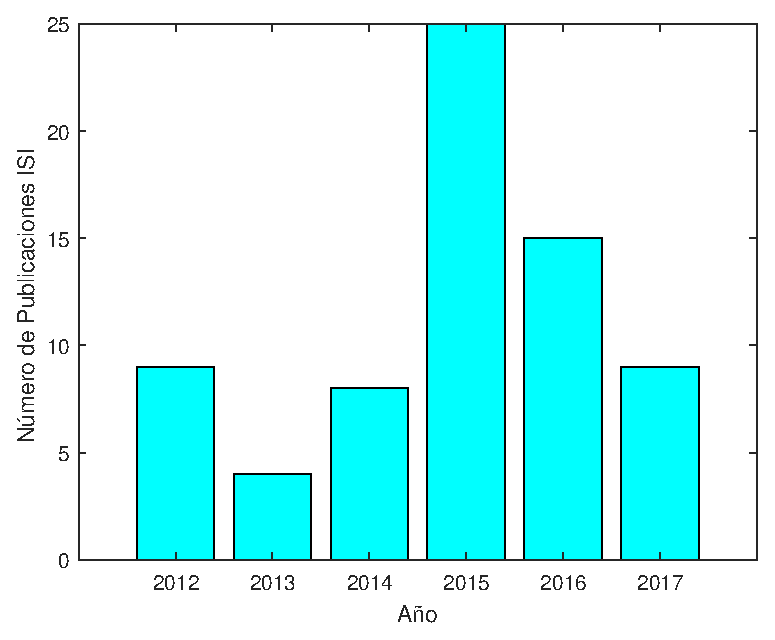
\includegraphics[width=0.7\columnwidth]{./pictures/publicaciones_ISI.eps}
\caption{Publicaciones con indexación ISI total de los profesores del claustro por año.}
\label{pub_isi}
\end{figure}

Adicionalmente en la encuesta (ver Sección \ref{academicos}) egresados y estudiantes del
Programa declaran 
estar entre muy de acuerdo y de acuerdo que el cuerpo académico
tiene una importante trayectoria, medido esto último en términos de publicaciones, participación
en proyectos, experiencia laboral y docencia. Es importante mencionar que los estudiantes evalúan a todo 
el cuerpo académico, no solo a los profesores del claustro. Lo que deja evidente el aporte de los colaboradores
al Programa.

\noindent Experiencia Laboral y Consultorías

El Programa cuenta con un claustro con bastante experiencia laboral. Los profesores del claustro
han trabajado en organizaciones como Bell Laboratories, Alcatel-Lucent, Sprint-Nextel, Nortel Networks,
Rockwell Collins, Federal Aviation Administration (FAA), People on Line, entre muchas otras organizaciones
internacionales trabajando en proyectos de telecomunicaciones. Aún con esta experiencia es importante mencionar 
el gran aporte que contribuye el cuerpo académico colaborador, donde gracias a estos profesores el Programa
reporta 30 consultas hechas en diversas organizaciones, hechas en el área de las telecomunicaciones.

\noindent Participación en Proyectos

Casi la totalidad de los miembros del claustro
lideran proyectos de investigación de forma permanente. Se destaca la participación de un 75\% del
claustro en Proyectos Fondecyt Regular e Iniciación (es decir, 3 de 4 académicos, donde los que
no tienen participación son académicos recientemente integrados). Además, los profesores mantienen numerosos
proyectos de transferencia y ciencia aplicada (Fondef, IDeA, entre otros). El total de proyectos en que participan 
los integrantes del claustro suma 26. El cuerpo académico colaborador 
también a participado en varios proyectos CORFO entre otros. 

\subsubsection{Crecimiento del Claustro e Incorporación de Académicos}

Adicionalmente a
la calidad de nuestra actividad es importante resaltar la renovación y crecimiento que ha
experimentado el claustro de Magíster en los últimos años, donde se constata la incorporación
de dos académicos en el 2017, que son Sandra Céspedes y Jinsong Wu. 
Esta política de renovación del cuerpo académico se enmarca en una plan
estratégico del Departamento de Ingeniería Eléctrica en mantener áreas balanceadas generando
las instancias administrativas formales que posibilitan la renovación del cuerpo académico. En
la actualidad se constata que un porcentaje significativo del cuerpo académico está compuesto
por académicos jóvenes (menores de 40 años), correspondiente al 50\% (2 de 4 académicos). 
Esta renovación posibilita una proyección del Programa en el mediano plazo. 


\subsubsection{Internacionalización del Cuerpo Académico}
\label{internacionalizacion}

Junto a la renovación del claustro en los últimos
años se destaca también su internacionalización. Actualmente (2017) todos los miembros 
del claustro son del extranjero, donde las nacionalidades son de los siguientes países: Venezuela,
Guatemala, Colombia y China). Cabe mencionar que dos profesores tienen ciudadanía de otros países (distintos 
a donde nacieron) y estos países son Chile y Canadá. Entre los colaboradores tenemos además la nacionalidad cubana.
Estos académicos tienen vínculos formales con instituciones extranjeras, junto con redes
de colaboración activas. Adicionalmente, todos los miembros del claustro obtuvieron
sus grados de Doctor en prestigiosas universidades internacionales (EEUU, Canadá y Korea del Sur) 
y gozan de numerosas redes de colaboración internacional.

\subsubsection{Cuerpo Académico Multidiciplinario}

Dado que el Programa tiene un perfil de egreso que incluye una gran variedad de destrezas industriales,
el cuerpo académico está incorporado por profesores que son expertos en leyes, economía, gestión de 
proyectos y de ciencias de la computación. Estos profesores permiten que el Programa pueda brindar 
conocimientos de regulación de las telecomunicaciones, análisis financieros, administración de proyectos y
temas de seguridad de redes. Esta gran diversidad de disciplinas es uno de los aspectos de los cuales
más nos enorgullece del Programa.

%\subsubsection{Consolidación de Académicos del Programa}

%En los últimos 5 años los académicos del claustro
%Pablo Estévez, Claudio Pérez, Javier Ruiz del Solar, Néstor Becerra y Martin Adams han sido
%nombrados en la más alta jerarquía académica de nuestra institución, Profesor Titular, como
%distinción a sus notables aportes a la institución en los ámbitos de formación (postgrado y
%pregrado), investigación y desarrollo. Esto constata la consolidación de los académicos con más
%experiencia en el Programa, hecho que repercute directamente en la jerarquía del cuerpo académico
%de éste y por ende en su consolidación en el tiempo. Dentro de los aportes notables de este
%grupo de académicos se destaca su importante rol en la formación de estudiantes en este Programa
%y en la formulación y ejecución de proyectos de investigación de gran envergadura de carácter
%interdisciplinario e Inter-universitario: Centro Basal AMTC, Fondap de Energía y proyecto Anillo.
%Además, los profesores Jorge Silva, Marcos Orchard, Doris Sáez y Patricio Mena han pasado de la
%jerarquía Profesor Asistente a Profesor Asociado.

%\subsubsection{Calidad y pertinencia del claustro}

%Los puntos analizados en la sección anterior dan cuenta de la calidad y pertinencia del claustro
%en virtud de los objetivos trazados en el Programa de Magíster. Se destaca una consolidación
%del claustro en el último tiempo y su renovación y proyección al mediano plazo. Se observa
%una presencia balanceada en todas las líneas de investigación que se cultivan en la disciplina de
%Ingeniera Eléctrica (Formulario de Acreditación Sección 4.2.3). Al mismo tiempo, la productividad
%creciente del claustro y la creciente participación en proyectos de investigación dan cuenta de un
%ecosistema rico en oportunidades para los estudiantes del Programa de magíster.

%\subsubsection{Evaluación del Sistema de Guías}

%Respecto al sistema de guía o seguimiento de los estudiantes, por diseño, la responsabilidad en
%primera instancia recae en la figura del profesor guía de tesis. Según el Reglamento General
%de Magíster [\ref{reg_mirc}], el Comité Académico nombra un guía desde la incorporación del estudiante
%el primer semestre. Los profesores guías están informados de los reglamentos de nuestros
%Programas, donde se estipulan entre otras cosas los objetivos, el plan de estudios, los objetivos de
%graduación, plazos y cumplimiento de compromisos formales (defensa de tesis). Adicionalmente
%a esto, el Coordinador del Programa vela por el cumplimiento del reglamento y se comunica
%directamente con los estudiantes del Programa para informar del reglamento y plazos. Se destaca
%las reuniones anuales de carácter informativo, dirigidas por el Coordinador del Programa y los
%comunicados enviados por el coordinador a los estudiantes para efectos de recordar el cumplimiento
%de plazos y obligaciones. Pese a lo anterior y en virtud de los tiempos de titulación y el análisis de
%casos donde no se ha dado cumplimiento a los plazos del Programa, se observa un espacio de mejora
%que propenda a un mejor seguimiento del progreso de los estudiantes y una mayor coordinación
%con los profesores guías de tesis.

\subsection{Definiciones Reglamentarias}

La Universidad de Chile, en su Reglamento General de Carrera Académica [\ref{reg_carrera}], establece tres
posibles Categorías Académicas:

\begin{enumerate}
\item La Categoría Académica Ordinaria, con cinco rangos consecutivos.
\item La Categoría Académica Docente, con tres rangos consecutivos.
\item La Categoría Académica Adjunta, con dos rangos.
\end{enumerate}

En particular, en el Departamento de Ingeniería Eléctrica de la Facultad de Ciencias Físicas
y Matemáticas, los académicos se encuentran adscritos a la Categoría Académica Ordinaria. De
acuerdo al Reglamento General de Carrera Académica, Artículo 6 [\ref{reg_carrera}]:

``Los académicos de la Categoría Académica Ordinaria deberán realizar docencia superior e
investigación o creación artística. Podrán, además, realizar otras de las actividades indicadas en
el artículo precedente, o una labor profesional destacada en el ámbito de su quehacer
académico.''

Adicionalmente el Reglamento General de estudios conducentes a los grados académicos de
Magíster y Doctor de la Universidad de Chile, párrafo 2, artículo 12 [\ref{reg_mag_doc}], establece que para la
creación de un Programa de magíster o doctorado:

``Cada Programa será desarrollado por un claustro conformado por académicos que cultiven las
disciplinas del Programa mediante investigación o creación artística original. El ingreso de un
académico al Claustro de un Programa será propuesto por el respectivo Comité Académico y
aprobado por el Consejo de la Escuela de Postgrado. La nómina actualizada de sus integrantes
será pública. Los académicos que integren el claustro de un Programa conducente al grado de
Magíster deberán ser profesores de cualquier carrera o categoría académica.''

Las normas básicas de la estructura, organización y administración del Programa se encuentran
estipuladas en el Reglamento General del Programa [\ref{reg_mirc}]. Es importante en este punto mencionar
que hay una nueva propuesta Reglamento General del Programa en proceso de revisión desde
el primer semestre del 2015. Adicionalmente, el Programa tiene un Reglamento Interno con
disposiciones específicas para regir el Programa dentro del marco otorgado por el Reglamento
General antes mencionado. Este reglamento es revisado periodicamente por el Comité Académico
del Programa, para ajustarlo a necesidades específicas de reglamentación interna, con el fin de
impulsar iniciativas de apoyo a los estudiantes, su seguimiento y, al mismo tiempo, facilitar la
gestión y coordinación del Programa.

\subsubsection{Del Comité Académico de Postgrado}

El Reglamento General de la Universidad de Chile [\ref{reg_mag_doc}] establece:

``El Programa constará de Comité Académico nombrado por el Director de Escuela de postgrado
de la FCFM a proposición del claustro académico del Programa, con el acuerdo del Consejo de
Escuela de la FCFM. En el mismo artículo se señala que el Comité estará conformado por al
menos tres miembros del claustro, quienes elegirán a uno de ellos como Coordinador. Será
responsabilidad del Comité gestionar los aspectos académicos del Programa, velando por el
cumplimiento de sus objetivos y por el mejoramiento continuo del Programa.''

Respecto a la gestión del Programa las funciones del Comité Académico, en concordancia con
el Reglamento General, corresponden a:

\begin{enumerate}
\item Seleccionar a los estudiantes que se incorporarán al Programa.
\item Aprobar los planes de estudios de los postulantes.
\item Nombrar a los respectivos profesores guías.
\item Aprobar al profesor guía de la tesis, propuesto por cada estudiante.
\item Proponer al Director de Escuela los integrantes de la Comisión Evaluadora de la Tesis.
\item Evaluar la calidad y originalidad del trabajo realizado y decidir si este alcanzó los
estándares requeridos para una Tesis de Magíster.
\item Elaborar un informe periódico sobre el estado del Programa, verificando el cumplimiento de
los indicadores de calidad definidos por la Facultad.
\item Cautelar que la investigación que realicen los estudiantes considere las normas y
procedimientos propios de la disciplina establecidas por los Comités de Ética respectivos
y/o reconocidos por la Universidad.
\end{enumerate}

\subsubsection{Del Ingreso, Permanencia y Evaluación del Claustro Académico}
\label{ing_perm_eval}

El Reglamento General de la Universidad de Chile [\ref{reg_mag_doc}] en su articulo 12 establece que:

``El ingreso de un académico al claustro, y su posterior permanencia, será propuesta por el Comité
Académico y aprobada por el Consejo de Escuela de Postgrado de la Facultad de Ciencias Físicas
y Matemáticas''.

La incorporación es solicitada por el académico interesado y posteriormente evaluada por el
Comité Académico en sus reuniones regulares, velando por el cumplimiento de la norma. Para
efectos de la permanencia en el claustro, el Comité evalúa anualmente el cumplimiento de los
criterios anteriormente señalados.

Adicionalmente a las disposiciones reglamentarias del Programa, los académicos del claustro
están subscritos a la carrera académica ordinaria (ver reglamento general de carrera académica
[\ref{reg_carrera}]). En este marco existen procesos permanentes de Calificación Académica, donde se
evalúa el desempeño general del académico considerando para ello docencia de pre y post grado,
investigación, tutoría de estudiantes, formación de profesionales y graduados, proyectos, gestión
docente, apoyo administrativo. Este proceso se ejecuta cada dos años para profesor de la jerarquía
de Profesor Asistentes y Asociados, y cada cuatro años para la jerarquía de Profesor Titular. Este
proceso exige que los académicos garanticen un buen cumplimiento en sus actividades académicas
y es un mecanismo formal a nivel institucional para evaluar a los académicos y condicionar su
permanencia en la institución en el caso que los criterios de permanencia mínimos exigidos en la
carrera académica ordinaria no sean satisfechos.

Complementando el punto anterior, en la Universidad de Chile hay un proceso de evaluación
académica que permite el paso de jerarquía académica (ver Reglamento Consejo Evaluación
[\ref{reg_cons_eval}]). Para ello los académicos deben cumplir con estrictos estándares de desempeño en lo
que respecta a la investigación y docencia, fundamentalmente. En este marco se estipula un tiempo
máximo de permanencia en la jerarquía de profesor asistente, que es de 10 años. Este tiempo
máximo de permanencia orienta la actividad de los profesores asistentes con miras a cumplir
estándares académicos que les permitan llegar a la jerarquía de Profesor Asociado en el plazo
señalado. Este proceso busca que los académicos pongan prioridad en actividades de investigación
y docencia de postgrado, de tal forma de mostrar independencia académica, liderar proyectos de
investigación como investigadores principales, y formar nuevas generaciones de profesionales y
académicos que cultiven su área del conocimiento.

\subsubsection{De la dedicación del claustro académico}

Como se explicó en la Sección \ref{ing_perm_eval}, los miembros
del claustro deben estar suscritos a la carrera académica ordinaria en el grado de profesor asistente,
asociado o titular. Por tanto todos los miembros del claustro tienen una dedicación de tiempo
completo a sus quehaceres académicos y docentes dentro de la universidad.

\subsubsection{Del sistema guías}

En concordancia con el reglamento general [\ref{reg_mag_doc}] en su artículo 26, al momento del ingreso del
estudiante al Programa la coordinación define su guía entre los académicos del claustro. Este
cumple el rol de orientar al estudiante en sus actividades académicas. Adicionalmente, para la
ejecución de la tesis el estudiante constará con un profesor guía de tesis nombrado por el Comité
Académico del Programa a proposición del estudiante, en concordancia con lo que establece el
Artículo 28 del mismo reglamento. El profesor guía de tesis debe pertenecer al claustro académico
del Programa.

\subsubsection{Evaluación docente}

Como parte de una política institucional de la FCFM, a través de la plataforma de U-Cursos, todos
los cursos cuentan con una encuesta para la evaluación docente de los profesores que se realiza
dos veces al semestre. Los resultados de esta evaluación son analizados en primera instancia por la
Jefatura Docente donde se determina si se debe ofrecer ayuda al profesor para la preparación del
curso junto con el área el departamento ADD. Por otro lado, los resultados de la encuesta forman
parte de todos los procesos de evaluación y cambio de jerarquía descritos en la Sección 2.4.3.2.

El sistema de profesores guías es evaluado en encuestas que se realizan previos al
proceso de acreditación. Una evaluación más rutinaria es necesaria. En la encuesta se observa que
la calificación dada por los estudiantes del Programa a sus profesores guías es
sobresaliente (ver Sección \ref{academicos}).

Un espacio de mejora en lo que refiere a tener información del desempeño de los profesores
guías de tesis, es hacer un evaluación más sistemática como se declara en el Plan de
Desarrollo de este proceso.

\subsubsection{Del seguimiento de los estudiantes}

El seguimiento de los estudiantes es una parte imprescindibles para la formación completa de los estudiantes. Como parte 
del seguimiento se tratan de detectar las debilidades en los conocimientos de los estudiantes en forma individual. A los 
estudiantes que exhiben debilidades se les trata de apoyar con distintos medios, por ejemplo: revisar las debilidades en 
la oficina del profesor, revisar las respuestas de las pruebas en la sala de clases, asignar tareas adicionales para que 
el estudiante practique, entre otros medios. La revisión de las pruebas luego de la examinación es beneficiosa tanto para 
los estudiantes de demostraron debilidades, tanto como para aquellos que mostraron dominio de los conceptos, ya que en este 
último caso la revisión de los resultados refuerza los conocimientos.

\section{Recursos de Apoyo}

\subsection{Apoyo Institucional e Infraestructura}
\label{apoyo_inst}

\subsubsection{Laboratorios y equipamiento}

El Programa cuenta con una amplia gama de laboratorios para la formación de sus estudiantes.
Efectivamente, el Departamento de Ingeniería Eléctrica posee tanto laboratorios docentes como de
investigación. Existen ocho laboratorios docentes especializados en diversos temas de ingeniería
eléctrica (ver detalles en Sección 5.1.2 del Formulario de Antecedentes del Programa):

\begin{itemize}
\item Laboratorio de Electricidad Básica,
\item Laboratorio de Automática,
\item Laboratorio de Accionamiento,
\item Energía y Electrónica de Potencia,
\item Laboratorio de Mecatrónica,
\item Laboratorio de Sistemas Inteligentes,
\item Laboratorio de Telecomunicaciones,
\item Laboratorio de Máquinas Eléctricas y
\item Laboratorio de Electrónica.
\end{itemize}

Estos son utilizados por los alumnos de pregrado y postgrado para completar su formación teórica.
Por otro lado existen 15 laboratorios de investigación donde estudiantes de pre y postgrado
realizan investigación:

\begin{itemize}
\item Laboratorio de Acumuladores,
\item Laboratorio de Control Avanzado,
\item Laboratorio de Energía y Accionamientos,
\item Laboratorio de Información y Decisión,
\item Laboratorio de Ingeniería Biomédica,
\item Laboratorio de Inteligencia Computacional,
\item Laboratorio de Micro Redes y Electromovilidad,
\item Laboratorio de Ondas Milimétricas y Submilimétricas,
\item Laboratorio de Procesamiento y Transmisión de Voz,
\item Laboratorio de Robótica, Laboratorio de Fotónica,
\item Optical \& Wireless Laboratory,
\item Laboratorio de Procesamiento Digital de Imágenes,
\item Laboratorio de Visión Computacional y
\item Laboratorio de Exploración Espacial y Planetaria.
\end{itemize}

En estos últimos los estudiantes de postgrado realizan la investigación y desarrollo relacionada a su trabajo
de tesis (Una descripción detallada de los laboratorios puede consultarse en el Formulario de
Acreditación Sección 5.1).

Todos los laboratorios cuentan con un responsable técnico y cuentan con un equipamiento
adecuado y en crecimiento. Las FCFM y el DIE garantizan la infraestructura básica de todos los
laboratorios. El financiamiento para la mantención y adquisición de nuevo equipamiento de los
laboratorios docentes es responsabilidad de la FCFM y del DIE. En el caso de los laboratorios
de investigación esta responsabilidad recae en el profesor o profesores líderes de cada laboratorio,
quienes recurren a fondos concursables.

\subsubsection{Recursos Bibliográficos}

Los estudiantes tienen acceso a una importante colección de recursos bibliográficos a través del
sistema de Bibliotecas de la Universidad10. Físicamente, se puede acceder a más de 120000 libros.
Además, a través de una moderna página web, se puede acceder electrónicamente a colecciones
de libros y revistas de conocidas casas editoriales. En particular, el DIE financia el acceso a la
colección de revistas de la IEEE, la más importante casa editorial de revistas científicas en diversas
áreas de la ingeniería eléctrica11. Respecto a las áreas más cercanas de investigación del Programa
podemos mencionar las siguientes subscripciones a revistas:

\begin{itemize}
\item 762 en Ingeniería Eléctrica en sí misma. En particular existe acceso a todas las revistas de
IEEE,
\item 145 en Tecnología de la Información,
\item 311 en Telecomunicaciones,
\item 118 en Física Aplicada,
\item 309 en Tecnología en General y
\item 111 en Astronomía y Astrofísica.
\end{itemize}

%\subsubsection{Becas y Ayudas de Viaje}

%En la actualidad el Programa cuenta con una rebaja arancelaria que equipara el arancel del
%Programa al fijado por Conicyt para sus becarios (actualmente \$1.000.000). Esta rebaja
%corresponde a un porcentaje importante del arancel anual del Programa. Este apoyo busca generar
%las condiciones favorables para que estudiantes que están participando en calidad de tesistas de un
%proyecto formal de investigación puedan pagar un arancel sustancialmente más bajo y por ende es
%un instrumento de apoyo a los estudiantes del Programa. Para esta ayuda se requiere autorización
%del tutor o profesor guía de tésis, quien solicita formalmente la ayuda al coordinador del Programa.

%En cuanto a las ayudas de viaje, esta es una dimensión donde se pueden hacer esfuerzos
%adicionales por mejorar. En el Plan de Desarrollo del presente proceso se elabora una nueva política
%para apoyar la participación de estudiantes del Programa en Congresos Internacionales. El criterio
%es que la conferencia sea de nivel mundial en su área de interés y que el estudiante presente un
%trabajo en calidad de primer autor. Este instrumento se comenzó a ejecutar el presente año 2015
%(ya se han hecho dos llamados a la fecha) y ha sido positivamente evaluado por los estudiantes
%activos del Programa como se constata en el ítem 7 de la encuesta (3.4.1).

\subsubsection{Vinculación con el Medio}
\label{vinculacion_medio}

El Programa tiene un vínculo con el medio a través de la investigación. Existen colaboraciones 
con científicos y organizaciones extranjeras a través de distintos proyectos e iniciativas. 
Un ejemplo de vinculación con el medio que se destaca es la colaboración 
que existe a través del proyecto ERANet-LAC. En este proyecto participan instituciones de 4 países de 
Latinoamérica y Europa. Los países que participan en este proyecto, a parte de Chile, son México,
Letonia y Romania.

Otra iniciativa internacional en que participaron todos los miembros del claustro y muchos colaboradores del Programa
fue una iniciativa llamada FOKUS, liderada por una organización alemana en Berlín, que tuvo participación de instituciones
académicas localizadas en Alemania, China y Tailandia, a parte de Chile.

Actualmente la Facultad cuenta con varios centros (mencionados en la Sección \ref{estruct_org_fcfm}) y 8 unidades de investigación
avanzada. A través de estos se realizan actividades de vinculación
con el sector productivo y la sociedad, con énfasis en la creación de conocimiento, desarrollo
y transferencia tecnológica. Cada uno es líder en su disciplina en el país. De estos centros
destacamos a continuación dos que son liderados por académicos del DIE y donde estudiantes del Magíster en Ingeniería de Redes de Comunicaciones ya han 
participado y donde otros tienen la oportunidad de participar.

\begin{itemize}
\item Centro Avanzado de Tecnología para la Minería (AMTC), Director: Dr. Javier Ruiz Del
Solar (DIE)
\item Centro de Investigaciones en Energía Solar (SERC-Chile), Director: Dr. Rodrigo Palma
Behnke (DIE)
\end{itemize}

Además, de todos estos vínculos también existen canales de colaboración con empresas como Entel
(en particular su rama de innovación), Telefónica I+D, 
Zweicom, ZTE Chile y ESIMTEL. Además de tener una buena relación con estas 
empresas, también han existido instancias de colaboración formal en proyectos FONDEF y CORFO.


\section{Capacidad de Autorregulación}

\subsection{Equilibrio entre estudiantes y recursos}

El Programa se ha caracterizado por velar por un adecuado equilibrio entre el número de estudiantes
matriculados y los recursos existentes. Prueba de ello es la consolidación del cuerpo académico. El
claustro del Magíster en Ingeniería de Redes de Comunicaciones, corresponde actualmente a
13 profesores contando los mismos del claustro y colaboradores. La cantidad de estudiantes 
activos en el Programa es de 13, lo que da una
razón promedio de 1 estudiantes por profesor. Esto es coherente con el hecho de que este es
un Programa orientado al desarrollo de competencias complejas en nuestros egresados, donde la
interacción personalizada con el profesor guía es esencial para lograr los objetivos del perfil
de egreso declarado.

Respecto a los recursos del Programa, en términos de laboratorios, biblioteca,
recursos bibliográficos, espacios de estudios, entre otros, éstos se caracterizan por su calidad
como se puede ver en detalle en la Sección \ref{apoyo_inst} de este informe. Como evidencia, la encuesta
a egresados, estudiantes y académicos muestra un amplio consenso respecto a la calidad del
Programa en lo que respecta a Apoyo Institucional e Infraestructura (ver Sección \ref{apoyo_inst_infra}). Sin
embargo, se aprecia un gran espacio de mejora en lo que respecta a laboratorios y/o talleres docentes
y la idoneidad de salas de clases para cumplir los requerimientos académicos. Cabe mencionar que se 
ha tenido dificultades con el equipo audiovisual (específicamente proyectores), probablemente 
debido a su extenso y constante uso, donde ha fallado en varias ocasiones. Se ha remplazado el equipo en al menos 
3 ocasiones en un periodo de 4 años. Es necesario estudiar el remplazo de estos equipos por una alternativa más duradera.
Esta ha sido una situación recurrente en el Programa.

En línea con el mejoramiento del Programa, es necesario tener mejoras con respecto al apoyo de
pasantías, congresos y otras actividades. A pesar de que el objetivo del Programa, ni el plan de
estudio exigen este tipo de actividades, sería idóneo poder financiarlos. Hay que estudiar bien 
la metodología, beneficios, recursos existentes y otros factores antes de ejecutar un plan 
(más detalles en el Plan de Desarrollo en la Sección \ref{plan_de_desarrollo}).

\subsection{Difusión}

La Universidad de Chile es particularmente cuidadosa en toda la entrega de información referente
a sus carreras y Programas de postgrado. En lo que se refiere a la difusión del Programa, se puede
mencionar la pagina web del DIE y MIRC como una plataforma con la información relevante del
Programa, su cuerpo académicos y otra informacióm importante. 
Acorde con esta política se han Programado visitas a universidades en la región al mismo modo que
solicitado a cada miembro del claustro del Programa que difunda el Programa en las conferencias y
seminarios internacionales en los que le toca participar regularmente. Otra instancia de difusión, es nuestra 
carta de presentación, o sea, nuestros egresados, que en un alto porcentaje declaran que recomendarían
el Programa a sus colegas y están satisfechos con la formación recibida del Programa.
Lo anterior se ve evidenciado por la alta apreciación y evaluación del Programa recogida en las
encuestas a egresados. % (ver Sección 3.4.1.9).

Complementariamente, parte de los esfuerzos de difusión del Programa son canalizados por
los medios oficiales de la Universidad de Chile a nivel de la Escuela de Postgrado y la Facultad.
En esto último, hay variadas actividades de difusión del quehacer de la Facultad donde se destacan
los días de puertas abiertas, la organización de charlas y seminarios, la publicación de la revista
Beaucheff, la página web de la Facultad y la Escuela de Postgrado. Es importante mencionar que
existe una unidad encargada de la difusión en la Facultad con recursos disponibles, Programas de
acción y personal administrativo dedicado a dichas tareas. En todos estos medios institucionales el
Departamento de Ingeniería Eléctrica ha mostrado una activa visibilidad. Actualmente la Escuela
de Postgrado realiza giras en Latinoamérica realizando difusión de toda la oferta de Postgrados de
la Facultad.

\subsection{Reglamentación}

La estructura reglamentaria de la Universidad de Chile es clara en lo que respecta a los Programas
conducentes a los grados de magister y doctorado [\ref{reg_mag_doc}]. Esta reglamentación define un marco
sobre el cual se regulan los Programas tocando aspectos tales como la naturaleza del Programa,
sus objetivos y perfil de graduación, su creación, la administración, la conformación del claustro,
las responsabilidades del comité académico, las responsabilidades de la escuela de postgrado, la
acreditación y procesos de aseguramiento de calidad. Adicionalmente en este Reglamento hay
disposiciones especificas para los Programas de Magister que tocan aspectos relativos a postulación
y criterios de selección, plan de formación, proyecto de grado, actividad de graduación, extensión
mínima y máxima del Programa, homologación de UDs, criterios de aprobación, entre otros.
Complementando lo anterior, el Programa mantiene un Reglamento General [\ref{reg_mirc}]. El Reglamento General del
Programa fue aprobado el 2016.


\subsection{Difusión de la Reglamentación}

Los reglamentos son públicos y de libre disposición para todos los miembros del Programa
(estudiantes y académicos). En particular, la pagina web del DIE mantiene dicha información
vigente. Sin embargo, el plan de desarrollo considera mejoras en este aspecto.

\subsection{Procesos de Diagnóstico}

El mejoramiento continuo y las instancias de diagnóstico se entienden como una parte esencial de
los Programas de postgrado que imparte la Universidad de Chile. En este marco, el Reglamento
General de la Universidad de Chile establece que los procesos de autoevaluación son parte esencial
de las responsabilidades del Comité Académico del Programa. Se establece que estos procesos
deben ser continuos y debe haber un proceso formal de revisión al menos cada 5 años. En
este contexto en los últimos años ha habido una serie de actividades e iniciativas de análisis y
diagnóstico participativas: Jornada de Escuela de Postgrado, Jornada estratégicas departamental
(Departamento de Ingeniería Eléctrica), análisis y revisión de los reglamentos del Programa,
reuniones con el claustro, así como las constantes reuniones del Comité Académico donde se
discuten aspectos operativos y estratégicos del Programa. A esto se suma el presente proceso de
autoevaluación del Programa. Adicionalmente el Programa consta con instrumentos de diagnóstico
que son utilizados regularmente para evaluarlo como son las Encuesta Docentes y el seguimiento
académico de sus estudiantes a través de la plataforma U-campus.

En el presente proceso, nuevas medidas han sido contempladas para el Plan de Desarrollo
donde se destaca la elaboración y toma de encuesta a la salida a los graduados del Programa y
la generación de informes anuales con indicadores que midan el desempeño del Programa. La
generación de estos insumos es importante para el análisis del Programa y con ello el desarrollo
futuro de éste.

\subsection{Plan de Desarrollo}

La elaboración y ejecución del plan de desarrollo se encuentra a cargo del Comité Académico
del Programa, liderado por su coordinador (artículo 17 Reglamento General [\ref{reg_mag_doc}]). Los recursos
para su ejecución provienen de recursos del Programa y del Departamento de Ingeniería Eléctrica.
En la ejecución del plan, el Comité recibe apoyo del equipo de gestión docente (jefe de estudios
y secretaria de postgrado). El plan de desarrollo que se desprende del presente proceso de
acreditación se presenta en forma detallada en el Capítulo 3 del presente informe.

\subsection{Autoevaluación y mejoramiento continuo}

Como se ha mencionado en el punto anterior, la Universidad de Chile es una institución fuertemente
autorregulada, dinámica y en mejora constante. Esto queda de manifiesto en las continuas mejoras
en todos los niveles institucionales y en diferentes dimensiones. Para mencionar algunas de las
instancias formales donde se generan los espacios de análisis y discusión de los Programas se
mencionan los procesos de autoevaluación, jornadas de análisis de postgrado a nivel institucional y
departamental, reuniones regulares del comité académico del Programa, procesos de actualización
periódica de los reglamentos, perfeccionamiento de instancias centrales como la Escuela de
Postgrado.
